\chapter{Background and Related Work}
\label{background}

This chapter summarises work that influences the design and implementation of 
the TAkka library.  It begins with a general introduction on the 
Actor programming model (Section~\ref{actor_general}) and the Supervision principle
(Section~\ref{supervision_principle}), then explains OTP design 
principles in Erlang (Section~\ref{erlang_otp}), followed by a short tutorial on how to use the Actor 
programming model and the Supervision principle in the Akka library (Section~\ref{akka_lib}).  The 
Chapter concludes with a summary of features of the Scala type system used in the TAkka 
implementation (Section~\ref{scala_essence}).  The Actor model makes concurrent programming easy.  The 
Supervision principle makes applications robust.  The Supervision principle is 
introduced in the Erlang language.  It is obligatory in the Akka library, 
which is implemented in the Scala language.  Scala has a sophisticated type 
system, which enabled the experimental building of the more powerful and 
easier-to-use library, TAkka.


\section{The Actor Programming Model}
\label{actor_general}

The Actor Programming Model was first proposed by \citet{Hewitt:1973} for the 
purpose of constructing concurrent systems.  In the model, a concurrent system
consists of actors which are primitive computational components. Actors 
communicate with each other by sending messages.  Each actor independently 
reacts to messages it receives.

The Actor model given in \citep{Hewitt:1973} does not specify its formal 
semantics and hence does not suggest implementation strategies either.  An 
operational semantics of the Actor model is developed by 
\citet{actor_operational_semantics}.  \citet{acot_laws} later define a set of 
axiomatic laws for Actor systems.  Other semantics of the Actor model include 
the denotational semantics given by \citet{actor_denotational_semantics} and 
the transition-based semantic model by \citet{actor_transition_semantic}.
Meanwhile, the Actor model has been implemented in Act 1 \citep{Act1}, a 
prototype programming language.  The model influences designs of 
Concurrency Oriented Programming Languages (COPLs), especially the Erlang 
programming language \citep{ArmstrongErlang}, which has been used in 
enterprise-level applications since it was developed in 1986.
  
A recent trend is adding actor libraries to full-fledged popular programming 
languages that do not have actors built-in.  Some of the recent actor libraries 
are JActor  \citep{JActor} for the JAVA language, Scala Actor \citep{actor_1, 
actor_2} for Scala, Akka \citep{akka_doc} for Java and Scala, and CloudHaskell 
\citep{CloudHaskell} for Haskell.


\section{The Supervision Principle}
\label{supervision_principle}

The core idea of the supervision principle is that actors should 
be monitored and restarted when necessary by their supervisors in order to 
improve the availability of a software system.  The supervision principle was 
first proposed in the Erlang/OTP library \citep{OTP} and was adopted by the Akka 
library \citep{akka_doc}.

A supervision tree in Erlang consists of two types of actors: workers and 
supervisors. A worker implements part of the business logic and reacts to 
request messages.  A supervisor is responsible for initializing and monitoring 
its children, which are workers or supervisors for other actors, and restarting 
its children when necessary.  The behaviour of a supervisor is defined by its 
{\it supervision strategy}.

The Akka library makes supervision obligatory.  In Akka, every user-created 
actor is either a child of the system guidance actor or a child of another 
user-created actor.  Therefore, every Akka actor is potentially the supervisor 
of some other actors.  Unlike the Erlang system, an Akka actor can be 
both a worker and a supervisor.





\section{Erlang and OTP Design Principles}
\label{erlang_otp}

Erlang \citep{erlang_history, ArmstrongErlang} is a dynamically typed 
functional programming language originally designed at the Ericsson Computer 
Science Laboratory for implementing telephony applications 
\citep{erlang_history}.  After using the Erlang language for in-house 
applications for ten years, when Erlang was released as open source in 1998, 
Erlang developers summarised five design principles shipped with the Erlang/OTP 
library, which stands for Erlang Open Telecom Platform \citep{erlang_history, 
OTP}.

Erlang provides fault-tolerant support for many enterprise-level distributed real-time
applications, which often contain components implemented using other languages.
One of the early OTP 
applications, Ericsson's AXD 301 switch, is reported to have achieved nine 9s 
availability, that is, 99.9999999\% of uptime, during its nine-month experiment 
\citep{ArmstrongAXD}.  Up to the present day, Erlang has been widely used in 
database systems (e.g. Mnesia, Riak, and Amazon SimpleDB) and messaging 
services (e.g. RabbitMQ and WhatsApp).


The five OTP design principles are: The Behaviour 
Principle, The Application Principle, The Release Principle, The Release 
Handling Principle, and The Supervision Principle \citep{OTP}.  The Supervision Principle 
was introduced in the previous section.  This section describes the ideas 
of the remaining 4 OTP design principles and the methodology of applying them 
in a JVM based environment, such as Java and Scala.  The Supervision principle, 
which is the central topic of this thesis, has no direct correspondence in 
general Java and Scala programming practice.



\subsection{The Behaviour Principle}

A Behaviour in Erlang is similar to an interface, a trait, or an abstract class
in object oriented programming.  It defines common structures and patterns of 
process implementations.  With the help of behaviours, Erlang code can be 
divided into a generic part (a behaviour module) and a specific part (a 
callback module).  Most Erlang processes, including those in the Erlang standard library,  are 
coded by implementing a set of pre-defined callback functions for one or 
more behaviours.  Although ad-hoc code and programming structures may be more 
efficient, using consistent general interfaces makes code more maintainable and 
reliable.  
\begin{comment}
Standard Erlang/OTP behaviours include: 

\begin{itemize} 
  \item $\it{gen\_server}$  for constructing the server of a client-server 
paradigm. 
  \item $\it{gen\_fsm}$ for constructing finite state machines. 
  \item $\it{gen\_event}$ for implementing event handling functionality. 
  \item $\it{supervisor}$ for implementing a supervisor in a supervision tree. 
\end{itemize}
\end{comment}

\newpage
\subsection{The Application Principle}

A software system on the OTP platform is made up of a group of components 
called applications.  To define an application, users implement two callback 
functions of the {\tt application} behaviour: {\tt start/2} and {\tt stop/1}.
In Erlang API, the signature of a function contains its name and the number
of arguments it takes.  Because Erlang is dynamically typed, users of an Erlang
library need to study the type of each function from respected documentation.
Applications without any processes are called library applications.  
In an Erlang runtime system, all operations on applications are managed by the 
$\it{application\ controller}$ process, registered as {\tt application\_controller}.

Distributed applications may be deployed on several distributed Erlang nodes.  
An Erlang distributed application will be restarted at another node when its 
current node goes down.  A distributed application is controlled by both the 
application controller and the distributed application controller, registered as 
{\tt dist\_ac}, both of which are part of the $\it{kernel}$  
application.  Two configuration parameters must be set before loading and 
launching a distributed application.  First, possible nodes where the 
distributed application may run must be explicitly pointed.  Second, all nodes 
configured in the last step will be sent a copy of the same configuration which 
includes three parameters: the time for other nodes to start, nodes that {\it 
must} be started in a timeout, and nodes that {\it may} be started in a 
timeout.


\subsection{The Release Principle and The Release Handling Principle}

A complete Erlang system consists of one or more applications, packaged in a 
release resource file.  Different versions of a release can be upgraded or 
downgraded at run-time dynamically by calling API in the {\tt release\_handler} 
module in the SASL (System Architecture Support Libraries) application.  Hot 
swapping on an entire release application is a distinct feature of Erlang/OTP, 
which aims at designing and running non-stop applications.


\subsection{Applying OTP Design Principles in Java and Scala}

To sum up, Table~\ref{otp} summarises an analogy between Erlang/OTP 
design principles and common practices in Java and Scala programming.  

\begin{table}[h]
\begin{tabular}{| l | p{10 cm} | }
\hline
  OTP Design Principle & Java/Scala Analogy \\
\hline
  Behaviour & defining an abstract class, an interface, or a trait. \\
\hline
  Application  & defining an abstract class that has two abstract methods: start 
and stop, or using Java/Scala an equivalent class such as {\tt Thread}. \\
\hline
  Release  & packaging related application classes  \\ 
\hline
  Release Handling  & hot swapping support on key modules is required \\
\hline
  Supervision  & no direct correspondence  \\
\hline
\end{tabular}
 \caption[]{Using OTP Design Principles in JAVA and Scala Programming}
\label{otp}
\end{table}

First, the notion of callback functions in Erlang/OTP is close to that
of abstract methods in Java and Scala.  An OTP behaviour that only defines the 
signature of callback functions can be ported to Java and Scala as an interface. 
 An OTP behaviour that implements some behaviour functions can be ported as an 
abstract class to {\it prevent} multiple inheritance, or a trait to {\it permit} 
multiple inheritance.  Since Java does not have the notion of trait, porting an 
Erlang/OTP module that implements multiple behaviours requires a certain amount 
of refactoring work.

Second, since the Erlang application module is just a special behaviour, a 
programmer can 
define an equivalent interface {\tt Application} which contains two abstract 
methods: {\tt start} and {\tt stop}.  To mimic the dynamic type system of Erlang 
system, the {\tt start} method may be declared as \\ 
{\tt public static void start(String name, Object... arguments)}
and as \\  
{\tt def start(name:String, arguments:Any*):Unit} in Java and Scala 
respectively. 

Third, Erlang releases correspond to  packages in Java and Scala whereas hot 
code swapping is not directly supported by JVM.  During the development of the 
TAkka library, the author noticed that dynamically upgrading key components can 
be mimicked by updating the references to those components.

The final OTP design principle, Supervision, has no direct correspondence in 
Java and Scala programming practices.  The next section introduces the Akka 
library which implements the supervision principle.






\begin{comment}

\section{The Erlang Programming Language}

Erlang \citep{erlang_history, ArmstrongErlang} is a dynamically typed 
functional programming language originally designed at the Ericsson Computer 
Science Laboratory for implementing telephony applications 
\citep{erlang_history}.  After using the Erlang language for in-house 
applications for ten years, when Erlang was released as open source in 1998, 
Erlang developers summarised five design principles shipped with the Erlang/OTP 
library, which stands for Erlang Open Telecom Platform \citep{erlang_history, 
OTP}.

Erlang, collaborates with other languages, provides fault-tolerant support for 
enterprise-level distributed real-time applications. One of the early OTP 
applications, Ericsson’s AXD 301 switch, is reported to have achieved nine “9”s 
availability, that is 99.9999999\% of uptime, during the nine months experiment 
\citep{ArmstrongAXD}.  Up to the present, 
Erlang has been widely used in database systems (e.g. Mnesia, Riak, and Amazon 
SimpleDB) and messaging services (e.g. RabbitMQ and WhatsApp).

This section gives a brief introduction to the Erlang programming language and 
OTP design principles, based on related material in \citep{ArmstrongErlang} and 
\citep{ErlangManual, ErlangStart, OTP}.




\subsection{Actor Programming in Erlang}

(This section summarises material from \citep[Chapter 8]{ArmstrongErlang} and 
\citep[Chapter 3]{ErlangStart})

\vspace{12 pt}

An Erlang application consists of one or more module files, each of which 
defines a set of functions.  The notion of the Erlang {\it process} minimizes 
the gap between sequential programming and concurrent programming.  In Erlang, 
a process is a thread of function execution.  It can receive messages of any 
type via its process identifier (pid).  Defining an Actor in Erlang is as 
simple as providing a {\tt receive} block for the body of the function spawned 
in a process.


\subsubsection{Processes Creation}

A {\it process} in Erlang is a thread of function execution.  A process is 
created by calling the {\tt spawn} method.  Figure~\ref{erlang_spawn} gives the 
API of the {\tt spawn} method \citep{ErlangManual}.  Calling {\tt spawn(Module, 
Function, Args)} creates a process that executes the function {\tt 
Module:Function(Args)}, where {\tt Args} is a list of arguments.  The {\tt 
spawn} method returns a process identifier (pid) of the created process, which 
terminates when the execution of the function completes.

\begin{figure}[!h]

\begin{lstlisting}
spawn(Module, Function, Args) -> pid()

  Module = Function = atom()
  Args = [Arg1,...,ArgN]  
  ArgI = term()
\end{lstlisting}  
\caption{Erlang API: spawn}
\label{erlang_spawn}
\end{figure}

To demonstrate the creation and usage of Erlang processes, Figure 
\ref{erlang_echo} shows the {\tt echo} example modified from \citep[the {\tt 
tut14} module]{ErlangStart} and its test result.  As the terminal output shows, 
the {\tt say\_something} function prints out its first argument for the number 
of times specified by its second argument.  What is more interesting is the 
result of {\tt echo:start()}, which spawns two processes.  The result shows 
that the execution of the two processes and the main thread, which returns a 
pid of the last {\tt spawn} (i.e. {\tt <0.41.0>}), are in parallel.  As a 
consequence, the program prints out ``hello'', ``goodbye'', and the pid in a 
non-deterministic order.

\begin{figure}[!h]
\begin{lstlisting}
-module(echo).

-export([start/0, say_something/2]).

say_something(_, 0) ->
    done;
say_something(What, Times) ->
    io:format("~p~n", [What]),
    say_something(What, Times - 1).

start() ->
    spawn(echo, say_something, [hello, 3]),
    spawn(echo, say_something, [goodbye, 3]).

%% Terminal Output:
%% 1> c(echo).
%% {ok,echo}
%% 2> echo:say_something(hello, 3).
%% hello
%% hello
%% hello
%% done
%% 3> echo:start().
%% hello
%% goodbye
%% <0.41.0>
%% hello
%% goodbye
%% hello
%% goodbye  
\end{lstlisting}  
\caption{Erlang Example: An Echo Process}
\label{erlang_echo}
\end{figure}



\subsubsection{Message Passing Style Concurrency}
\label{erlang_message_passing}
In the {\tt echo} example, the two processes are executed independently.  To 
be an actor, an Erlang process shall be able to receive messages from others 
and reacts to messages.

In Erlang, users can send a message to a process via its pid using the {\tt !} 
primitive.  For example, the code 
\begin{lstlisting}
  Pid ! Msg
\end{lstlisting}
will send the message {\tt Msg} to the process whose pid is {\tt Pid}. Message 
sending is an asynchronous operation. Its evaluation result is the evaluated 
value of the sent message.

Messages sent to a process is queued in the mailbox of the recipient.  To 
handle a received message, a process provides a {\tt receive} block with the 
following syntax:

\begin{figure}[h]
\begin{lstlisting}
 receive
   Message1 [when Guard1] ->
     Action1 ;
   Message2 [when Guard2] ->
     Action2 ;
   ...
   MessageN [when GuardN] ->
     ActionN
 end
\end{lstlisting}
\caption{Erlang receive block}
\label{fig:ErlangReceiveAPI}
\end{figure}

In the Erlang code pattern given in Figure~\ref{fig:ErlangReceiveAPI}, {\tt 
receive} and {\tt end} are primitives that denote the scope of the receive 
block.  A receive block defines a set of guarded message patterns to which the 
current processed message will be matched in order. If the current message 
matches a pattern, the corresponding action will be evaluated.  If the current 
message does not match any pattern, it will be saved in the mailbox and the 
next message in the mailbox will be processed.  When reaching a receive block, 
the evaluation of the process will be suspended until at least one message in 
the mailbox matches one of the guarded patterns.  

Because messages may be concurrently sent from parallel threads or distributed 
nodes, the order in which messages appear in the mailbox 
is not necessarily the same as the order those messages were sent.  
Nevertheless, messages sent from the same sender to the same receiver is 
guaranteed to appear in the mailbox in the order they were sent, if both are 
delivered.     

The {\tt echo\_actor} example, given in Figure~\ref{fig:ErlangEchoActor}, 
spawns two processes, both of which verbatim print their received messages.  
The {\tt print} function terminates as soon as the first message is processed.  
On the contrary, {\tt loop} is a recursive function that can always process new
messages.  Line 34 of Figure~\ref{fig:ErlangEchoActor} confirms two properties 
of message sending in Erlang.  Firstly, message sending is always a successful 
operation that returns the value of the sent message.  At line 24, {\tt P} is a 
pid pointing to a terminated process.  Nevertheless, sending a message to {\tt 
P} is still permitted.  Secondly, message sending  is an asynchronous operation. 
 In this example, the evaluation result of line 23 is printed out after the 
evaluation result of the {\tt start} function (i.e. {\tt hello4}), probably 
because it takes some time to match the message sent in line 23.





\begin{figure}[!h]

\begin{lstlisting}
-module(echo_actor).

-export([start/0, loop/0, print/0]).

loop() ->
    receive
        Msg -> 
          io:format("loop: ~p~n", [Msg]),
          loop()
    end.

print() ->
    receive
        Msg -> 
          io:format("print: ~p~n", [Msg])
    end.
    
start() ->
    L = spawn(echo_actor, loop, []),
    P = spawn(echo_actor, print, []),
    L ! hello1,
    P ! hello2,
    L ! hello3,
    P ! hello4.


%% Terminal Output:

%% 1> c(echo_actor).     
%% {ok,echo_actor}
%% 2> echo_actor:start().
%% loop: hello1
%% print: hello2
%% hello4
%% loop: hello3


\end{lstlisting}
\caption{Erlang Example: An Echo Actor}
\label{fig:ErlangEchoActor}
\end{figure}


\subsubsection{An Erlang Actor with State}

Erlang is a functional programming language where the value of a variable is 
immutable once assigned.  On the other side, the result of a computation, for 
example, a search query, often depends on the value of some internal states.  
Therefore, an Erlang actor needs to retain or update its internal states when it
updates its behaviour.  One common method to define an Erlang actor with 
internal
state is passing the state to the behaviour function.  


The {\tt counter} example defined in Figure~\ref{fig:erlang_counter} has one 
state variable, {\tt Val}, which records the number of messages it has 
processed.  The internal state is initialized to 0 when the actor is 
created at line 5.  The value of the state is incremented each time when a 
message is processed (line 14 and line 17).

\begin{figure}[!h]


\begin{lstlisting}
-module(counter).
-export([start/0, counter/1]).
 
start() ->
    S = spawn(counter, counter, [0]),
    S ! increment,
    send_msgs(S, 3),
    S.
 
counter(Val) ->
    receive
        increment ->
          io:fwrite("increase counter to ~w~n", [Val+1]),
          counter(Val+1);
        Msg -> 
          io:fwrite("~w message(s) that has/have been processed ~n", [Val+1]),
          counter(Val+1)
    end.
 
send_msgs(_, 0) -> true;
send_msgs(S, Count) ->
    S ! "Hello",
    send_msgs(S, Count-1).
 
%% Terminal Output:
%% 1> c(counter).
%% {ok,counter}
%% 2> counter:start().
%% increase counter to 1
%% <0.95.0>
%% 2 message(s) has/have been processed 
%% 3 message(s) has/have been processed 
%% 4 message(s) has/have been processed
\end{lstlisting}
  \caption{Erlang Example: A Message Counter}
  \label{fig:erlang_counter}
\end{figure}



\subsection{Supervision in Erlang}
\label{erlang_supervision}

(This section summarises material from \citep[Chapter 5]{OTP})
\vspace{12 pt}

Supervision is probably the most important concept in the OTP design 
principles \citep{OTP}.  A supervision tree consists of workers and 
supervisors. Workers are processes which carry out actual computations while 
supervisors are processes which inspect a group of workers or sub-supervisors.  
Since both workers and supervisors are processes and they are organised in a 
tree structure, the term $\it{child}$ is used to refer to any supervised 
process.  The structure of a supervision tree may look like the 
one presented in Figure~\ref{fig:erlang_supervison_tree}, where supervisors are 
represented by squares and workers are represented  by circles.  The example is 
cited from \citep[Section 1.1]{OTP}.  Restart strategies of each supervisor 
(Section~\ref{erlang_supervision_strategy}), however, are 
removed from the figure since they are not related to the central ideas 
discussed at this moment.

\vspace{12 pt}

\begin{figure}[h]
\begin{center}

\begin{picture}(280, 250)
  \put(15, 70){\circle{30}}
  \put(95, 0){\circle{30}}
  \put(180, 0){\circle{30}}
  \put(260, 0){\circle{30}}
  
  \put(80,55){\line(0,1){30}}
  \put(80,85){\line(1,0){30}}
  \put(110,85){\line(0,-1){30}}
  \put(110,55){\line(-1,0){30}}
  
  \put(200,55){\line(0,1){30}}
  \put(200,85){\line(1,0){30}}
  \put(230,85){\line(0,-1){30}}
  \put(230,55){\line(-1,0){30}}
  
  \put(140,125){\line(0,1){30}}
  \put(140,155){\line(1,0){30}}
  \put(170,155){\line(0,-1){30}}
  \put(170,125){\line(-1,0){30}}
  
  \put(0,125){\line(0,1){30}}
  \put(0,155){\line(1,0){30}}
  \put(30,155){\line(0,-1){30}}
  \put(30,125){\line(-1,0){30}}  

  \put(70,202){\line(0,1){30}}
  \put(70,232){\line(1,0){30}}
  \put(100,232){\line(0,-1){30}}
  \put(100,202){\line(-1,0){30}}  

  \put(180,15){\line(1,1){40}}
  \put(260,15){\line(-1,1){40}}
  \put(95,15){\line(0,1){40}}
  
  \put(95,85){\line(3,2){62}}
  \put(220,85){\line(-3,2){62}}
  \put(15,85){\line(0,1){40}}
  
  \put(15,155){\line(3,2){70}}
  \put(155,155){\line(-3,2){70}}
\end{picture}

\end{center}
\caption{A Supervision Tree}
\label{fig:erlang_supervison_tree}
\end{figure}

\newpage

\subsubsection{An Erlang Supervision Example}

We present the code for a simple Erlang supervisor in Figure 
\ref{erlang_supervision_demo}.  The core computation of the {\tt 
supervision\_demo} example is a problematic function {\tt loop}, which 
eventually will try to compute the quotient of 10 divided by 0.  As the test 
result shows, the problematic process has been restarted twice when it raises 
an error.  The process is killed when it has failed for the third time within 
60 seconds.  

The short example implements the {\tt supervisor} behaviour and specifies its 
supervision policy in its {\tt init/1} method.  The supervision policy 
reads as the following: spawn a worker process by calling {\tt 
spawn(supervisor\_demo, start, [Count])}; always restart the child when it 
fails if it does not fail more than twice within 60 seconds; if the 
child process fails more frequently than allowed, terminate it immediately.  
Alternative Erlang supervision strategies are explained in the following.

\begin{figure}[p]

\begin{lstlisting}
-module(supervisor_demo).
-behaviour(supervisor).

-export([start/0, start/1, loop/1, init/1]).

start() ->
    supervisor:start_link(supervisor_demo, [2]).

start(Count) ->
  io:fwrite("Starting...~n"),
  Pid=spawn_link(supervisor_demo, loop, [Count]),
  {ok, Pid}.
	
init([Count]) ->
  {ok, {{one_for_one, 2, 60},
          [{supervisor_demo, {supervisor_demo, start, [Count]},
          permanent, brutal_kill, worker, [supervisor_demo]}]}}.
	
loop(Count) ->
  io:fwrite("~w / ~w is ~w ~n", [10, Count, 10/Count]),
  loop(Count-1).
  
%% 1> c(supervisor_demo).
%% {ok,supervisor_demo}
%% 2> supervisor_demo:start().
%% Starting...
%% 10 / 2 is 5.0 
%% 10 / 1 is 10.0 
%% <0.39.0>
%% Starting...
%% 10 / 2 is 5.0 
%% 10 / 1 is 10.0 
%% Starting...
%% 3> 
%% =ERROR REPORT==== 14-Oct-2013::00:03:49 ===
%% Error in process <0.40.0> with exit value: 
{badarith,[{supervisor_demo,loop,1,[{file,"supervisor_demo.erl"},{line,20}]}]}
%% 10 / 2 is 5.0 
%% 3> 
%% =ERROR REPORT==== 14-Oct-2013::00:03:49 ===
%% Error in process <0.42.0> with exit value: 
{badarith,[{supervisor_demo,loop,1,[{file,"supervisor_demo.erl"},{line,20}]}]}
%% 10 / 1 is 10.0 
%% =ERROR REPORT==== 14-Oct-2013::00:03:49 ===
%% Error in process <0.43.0> with exit value: 
{badarith,[{supervisor_demo,loop,1,[{file,"supervisor_demo.erl"},{line,20}]}]}
%% ** exception error: shutdown
\end{lstlisting}  
\caption{Erlang Example: Supervision Demo}
\label{erlang_supervision_demo}
\end{figure}




\subsubsection{Supervision Strategy}
\label{erlang_supervision_strategy}

In principle, a supervisor is accountable for starting, stopping and monitoring 
its child processes according to the policy specified in its {\tt init/1} 
method, according to the API given in Figure~\ref{erlang_supervision_api} 
\citep{OTP}.  A supervision strategy contains two parts: a restart strategy 
applies to all children and a list of child specifications for each child.

An Erlang supervisor employs one of the four restart strategies which specify 
its behaviour when one of its child fails.  A supervisor with {\tt 
one\_for\_one} strategy restarts a child when it fails.  A supervisor with {\tt 
one\_for\_all} strategy restarts all children when one of them fails.  A 
supervisor with {\tt rest\_for\_one} strategy restart the failed child and 
other children that started later than the failed child, according to their 
order in the list of child specifications.  A supervisor with 
{\tt simple\_one\_for\_one} strategy is a {\tt one\_for\_one} supervisor whose 
children are dynamically added instances of the same process.

A child specification contains 6 pieces of information \citep{OTP}: 
\begin{inparaenum} [i)]
  \item an internal name of the supervisor to identify the child. 
  \item the function call to start the child process.
  \item whether the child process should be restarted after the termination of 
its siblings or itself.
  \item how to terminate the child process.
  \item whether the child process is a worker or a supervisor.
  \item a singleton list which specifies the name of the callback module. 
\end{inparaenum}



\begin{figure}[p]

\begin{lstlisting}
Module:init(Args) -> Result

Args = term()
Result = {ok, {{RestartStrategy,MaxR,MaxT},[ChildSpec]}} | ignore
   RestartStrategy = strategy()
   MaxR = integer()>=0
   MaxT = integer()>0
   ChildSpec = child_spec()
   
child_spec() = 
    {Id :: child_id(),
     StartFunc :: mfargs(),
     Restart :: restart(),
     Shutdown :: shutdown(),
     Type :: worker(),
     Modules :: modules()}
     
child_id() = term()

mfargs() = 
    {M :: module(), F :: atom(), A :: [term()] | undefined}

restart() = permanent | transient | temporary

shutdown() = brutal_kill | timeout()

strategy() = one_for_all
           | one_for_one
           | rest_for_one
           | simple_one_for_one
               
worker() = worker | supervisor            

modules() = [module()] | dynamic

\end{lstlisting}  
\caption{Erlang API: supervision}
\label{erlang_supervision_api}
\end{figure}



\subsection{Other OTP Design Principles}

Based on 10 years of experience of using Erlang in Enterprise level 
applications, Erlang developers summarized 5 OTP design principles in 1999 to 
improve the reliability of Erlang applications \citep{OTP}: The Behaviour 
Principle, The Application Principle, The Release Principle, The Release 
Handling Principle, and The Supervision Principle.  The Supervision Principle 
has been introduced in the previous section.  This section describes the idea 
of the remaining 4 OTP design principles and the methodology of applying them 
in a JVM based environment, such as Java and Scala.  The Supervision principle, 
which is the central topic of this thesis, has no direct correspondence in 
general Java and Scala programming practice.

\subsubsection{The Behaviour Principle}

A Behaviour in Erlang is similar to an interface, a trait, or an abstract class
in the objected oriented programming.  It implements common structures and patterns of process 
implementations.  With the help of behaviours, Erlang code can be divided into a 
generic part, a behaviour module, and a specific part, a callback module.  Most 
processes, including the supervisor in Section~\ref{erlang_supervision}, is coded
by implementing a set of pre-defined callback functions for one or 
more behaviours.  Although ad-hoc code and programming structures may be more 
efficient, using consistent general interfaces make code more maintainable and 
reliable.  Standard Erlang/OTP behaviours include: 

\begin{itemize} 
  \item $\it{gen\_server}$  for constructing the server of a client\-server 
paradigm. 
  \item $\it{gen\_fsm}$ for constructing finite state machines. 
  \item $\it{gen\_event}$ for implementing event handling functionality. 
  \item $\it{supervisor}$ for implementing a supervisor in a supervision tree. 
\end{itemize}


\subsubsection{The Application Principle}

A software system on the OTP platform is made of a group of components called 
applications.  To define an application, users implements two callback 
functions of the {\tt application} behaviour: {\tt start/2} and {\tt stop/1}.  
Applications without any processes are called library applications.  
In an Erlang runtime system, all operations on applications are managed by the 
$\it{application\ controller}$ process, registered as {\tt application\_controller}.

Distributed applications may be deployed on several distributed Erlang nodes.  
An Erlang distributed application will be restarted at another node when its 
current node goes down.  A distributed application is controlled by both the 
application controller and the distributed application controller, registered as 
{\tt dist\_ac}, both of which are part of the $\it{kernel}$  
application.  Two configuration parameters must be set before loading and 
launching a distributed application.  First, possible nodes where the 
distributed application may run must be explicitly pointed.  Second, all nodes 
configured in the last step will be sent a copy of the same configuration which 
include three parameters: the time for other nodes to start, nodes that {\it 
must} be started in a given time, and nodes that {\it may} be started in a 
given time.


\subsubsection{The Release Principle and The Release Handling Principle}

A complete Erlang system consists of one or more applications, packaged in a 
release resource file.  Different version of a release can be upgraded or 
downgraded at run-time dynamically by calling API in the {\tt release\_handler} 
module in the SASL (System Architecture Support Libraries) application.  Hot 
swapping on an entire release application is a distinct feature of Erlang/OTP, 
which aims at design and running non-stop applications.


\subsubsection{Appling OTP Design Principles in Java and Scala}

To sum, we make an analogy between Erlang/OTP design principles and common 
practices in Java and Scala programming, summarised in Table~\ref{otp}.  

\begin{table}[h]
\begin{tabular}{| l | p{10 cm} | }
\hline
  OTP Design Principle & Java/Scala Analogy \\
\hline
  Behaviour & defining an abstract class, an interface, or a trait. \\
\hline
  Application  & defining an abstract class that has two abstract methods: start 
and stop \\
\hline
  Release  & packaging related application classes  \\ 
\hline
  Release Handling  & hot swapping support on key modules is required \\
\hline
  Supervision  & no direct correspondence  \\
\hline
\end{tabular}
 \caption[]{Using OTP Design Principles in JAVA and Scala Programming}
\label{otp}
\end{table}

First, the notion of callback functions in Erlang/OTP is close to the notion 
of abstract methods in Java and Scala.  An OTP behaviour that only defines the 
signature of callback functions can be ported to Java and Scala as an interface. 
 An OTP behaviour that implements some behaviour functions can be ported as an 
abstract class to {\it prevent} multiple inheritance, or a trait to {\it permit} 
multiple inheritance.  Since Java does not have the notion of trait, porting an 
Erlang/OTP module that implements multiple behaviours requires a certain amount 
of refactoring work.

Second, since the Erlang application module is just a special behaviour, we can 
define an equivalent interface {\tt Application} which contains two abstract 
methods: {\tt start} and {\tt stop}.  To mimic the dynamic type system of Erlang 
system, the {\tt start} method may be declared as \\{\tt public static void 
start(String name, Object... arguments)}  and as \\  
{\tt def start(name:String, arguments:Any*):Unit} in Java and Scala 
respectively. 

Third, Erlang releases correspond to  packages in Java and Scala whereas hot 
code 
swapping is not directly supported by JVM.  During the development of the TAkka 
library, we noticed that hot code swapping on a key component can be mimicked 
by updating the reference to that component.

The final OTP design principle, Supervision, has no direct correspondence in 
Java and Scala programming practices.  The next section introduces the Akka 
library which implements the supervision principle.


\end{comment}




\section{The Akka Library}
\label{akka_lib}

Akka is a Scala library that enforces the supervision principle.  The next section briefly
introduces Scala features that used in this thesis.  The API of the 
Akka library \citep{akka_api, akka_doc} is similar to the Scala 
Actor library \citep{actor_1, actor_2}, which borrows syntax from the Erlang 
languages \citep{ArmstrongErlang, ErlangManual}.  Both Akka and Scala Actor are 
built in Scala, a typed language that merges features from Object-Oriented 
Programming and Functional Programming.  This section gives a brief tutorial 
on Akka, based on related materials in the Akka Documentation 
\citep{akka_doc}.  The Akka API used in this thesis is listed in Figure A.1, Appendix A.


\subsection{Actor Programming in Akka}
\label{subsection:actor_akka}

(This section summarises material from \citep[Section 2.3 and 3.1]{akka_doc})
\vspace{12 pt}

Although many Akka designs have their origin in Erlang, the Akka Team at 
Typesafe Inc. devises a set of connected concepts that explains Actor 
programming in the Akka framework.  This subsection begins with a short Akka 
example, followed by elaborate explanations of involved concepts.



\begin{figure}[p]
      \begin{lstlisting}[language=scala]
package sample.akka

import akka.actor.{Actor, ActorRef, ActorSystem, Props}
      
class StringCounter extends Actor {
  var counter = 0;
  def receive = {
    case m:String => 
      counter = counter +1
      println("received "+counter+" message(s):\n\t"+m)
  }
}

class MessageHandler extends Actor {
  def receive = {
    case akka.actor.UnhandledMessage(message, sender, recipient) =>
      println("unhandled message:"+message);
  }
}

object StringCounterTest extends App {
  val system = ActorSystem("StringCounterTest")
  val counter = system.actorOf(Props[StringCounter], "counter")
  
  val handler = system.actorOf(Props[MessageHandler]))
  system.eventStream.subscribe(handler,classOf[akka.actor.UnhandledMessage]);
  counter ! "Hello World"
  counter ! 1
  Thread.sleep(1000)
  val counterRef = system.actorFor("akka://StringCounterTest/user/counter")
  counterRef ! "Hello World Again"
  counterRef ! 2
}


/*
Terminal output:
received 1 message(s):
	Hello World
unhandled message:1	
received 2 message(s):
	Hello World Again
unhandled message:2
*/
    \end{lstlisting}
    \caption{Akka Example: A String Counter}
 \label{fig:akka_string_counter}    
\end{figure}

The code presented in Figure~\ref{fig:akka_string_counter} defines and uses an
actor which counts String messages it receives.  An Akka actor implements its 
message handler by defining a {\tt receive} method of type 
{\tt PartialFunction[Any, Unit]}.  In Scala, {\tt Any} is the supertype of all types.  
The type {\tt Unit} has a unique value, {\bf ()}.  A method with the return 
type {\tt Unit}, such as the  {\tt receive} method, represents a block of local 
actions.  Analogous to such a method is a Java method which is declared {\tt 
void}. In the {\tt StringCounterTest} application, we create an Actor System 
(Section~\ref{akka_actor_system}), initialise an actor (Section~\ref{akka_actor_class}) 
inside the Actor System by passing a corresponding {\tt Props} (Section~\ref{akka_props}),
and send messages to the created actor via its actor references (Section~\ref{akka_actor_reference}).
Unexpected messages to the {\tt counter} actor (e.g. line 28 and 31) are handled
by an instance of {\tt  MessageHandler}, a helper actor for the test 
application. 


\subsubsection{Actor System}
\label{akka_actor_system}

In Akka, every actor is resident in an Actor System.  An actor system organises 
related actors in a tree structure and provides services such as thread  
scheduling, network connection, and logging.  One or several local and remote 
actor systems constitute a complete application.  

To create an actor system, users provide a  name and an optional configuration 
to the {\tt ActorSystem} constructor.  For example, an actor system is created 
in Figure  
\ref{fig:akka_string_counter} by the following code. 
\begin{lstlisting}[language=scala]
  val system = ActorSystem("StringCounterTest")
\end{lstlisting}

In the above, an actor system of name \textcolor{mauve}{StringCounterTest} is 
created in the machine where the program runs.  The above created actor system 
uses the default Akka system configuration which provides a simple logging 
service, a round-robin style message router, but does not support remote 
messages.  Customized configuration can be encapsulated in a {\tt Config} 
instance and passed to the {\tt ActorSystem} constructor, or specified as part 
of the application configuration file.  This short tutorial will not look into 
customized configurations, which have minor differences in different Akka 
versions, and are not related to the central topics of this thesis.

\subsubsection{The Actor Class}
\label{akka_actor_class}

An Akka Actor has four groups of fields given in Figure~\ref{akka_actor_api}:
\begin{inparaenum}[\itshape i\upshape)]
\item its {\it state}, 
\item its {\it behaviour} functions, 
\item an {\tt ActorContext} instance encapsulating its contextual information,  and
\item the {\it supervisor strategy} for its children. 
\end{inparaenum}
This subsection explains the {\it state} and {\it behaviour} of actors, which 
are required when defining an Actor class.  Overriding default {\it actor 
context} and {\it supervisor strategy} will be explained in later subsections.

\begin{figure}[h]
\begin{lstlisting}[language=scala]
trait Actor extends AnyRef
  type Receive = PartialFunction[Any, Unit]
  
  abstract def receive: Actor.Receive
  implicit final val self: ActorRef  
  implicit val context: ActorContext
  def supervisorStrategy: SupervisorStrategy
  
  final def sender: ActorRef
  
  def preStart(): Unit
  def preRestart(reason: Throwable, message: Option[Any]): Unit
  def postRestart(reason: Throwable): Unit  
  def postStop(): Unit}
\end{lstlisting}
\caption{Akka API: Actor}
\label{akka_actor_api}
\end{figure}

An Akka actor may contain some mutable variables and immutable values that 
represent its {\it internal state}.  Each Akka actor has an actor reference, 
{\tt self}, through which messages can be sent to that actor.  The value of 
{\tt 
self} is initialised when the actor is created. Notice that {\tt self} is 
declared as a value field ({\tt val}), rather than a variable field 
({\tt var}), so that its value cannot be changed.  In addition to {\it 
immutable 
states}, sometimes {\it mutable states} are also required.  For example, Akka 
developers decided that the sender of the last message should be recorded and 
easily fetched by calling the {\tt sender} method.  In the {\tt StringCounter} 
example, we straightforwardly add a {\tt counter} variable which is initialized 
to 0 and is incremented each time a String message is processed.

There are two drawbacks to using mutable internal variables to represent 
states. Firstly, those variables will be reset each time when the actor is 
restarted, either due to a failure caused by itself or be enforced by its 
supervisor for other reasons.  Secondly, mutable internal variables result in 
the difficulty of implementing a consistent cluster environment where actors may 
be replicated to increase reliability \citep{Kuhn12}.  Alternatives to 
working with mutable states will be discussed in Section 
\ref{alternative_designs}.

There are two kinds of {\tt behaviour} functions of an actor.  The first type of 
behaviour function is a {\tt receive} function which defines its action to 
incoming messages.  The {\tt receive} function is declared as an {\tt abstract} 
function, which must be implemented otherwise the class cannot be initialised. 
The second group of behaviour functions has four overridable functions which 
are triggered before the actor is started ({\tt preStart}), before the actor is 
restarted ({\tt preRestart}), after the actor is restarted ({\tt postRestart}), 
and when the actor is permanently terminated ({\tt postStop}). The default 
implementation of those four functions take no action when they are 
invoked.

Upon close inspection, it can be seen that the {\tt receive} function of the 
{\tt StringCounter} actor in Figure~\ref{fig:akka_string_counter} actually 
has type {\tt Function[String, Unit]} rather than the declared type {\tt 
PartialFunction[Any, Unit]}.  The definition  of {\tt StringCounter} is 
accepted by the Scala because {\tt PartialFunction} does not check the 
completeness of the input patterns.  The behaviour of processing non-String 
messages, however, is undefined in the {\tt receive} method.

\subsubsection{Message Mailbox}
\label{message mailbox}

An actor receives messages from other parts of the application.  Arriving 
messages are queued in its sole mailbox to be processed.  Differently to the 
Erlang design, the behaviour function of 
an Akka actor must be able to process the message it is given.  If the message 
does not match any message pattern of the current behaviour, a failure arises.

Undefined messages are treated differently in different Akka versions.  In
versions prior to 2.0, an Akka actor raises an exception when it processes an 
undefined message. It means that sending an ill-typed message will cause a 
failure at the receiver side.  In Akka 2.1, an undefined message is discarded 
by the actor and an {\tt UnhandledMessage} event is pushed to the event stream 
of the actor system. The event stream may be subscribed to by other actors who 
are interested in particular event messages.  Line 24 of the String Counter
example demonstrates how to subscribe to messages in the event stream
of an actor system.




\begin{comment}
In Akka 2.2, the {\tt 
Stash} trait can be used to pending the process of a particular message until 
the current behaviour is updated.
\end{comment}



\subsubsection{Actor Creation with Props}
\label{akka_props}

An instance of the {\tt Props} class, which presumably stands for ``properties'', 
specifies the configuration used in creating an actor. A {\tt Props} instance 
is immutable so that it can be consistently shared between threads and 
distributed nodes.  

Figure~\ref{akka_props_api} gives part of the API of the {\tt Props} class and 
its companion object.  The {\tt Props} class is defined as a {\it final class} 
so that 
users cannot define subclasses of it.  Moreover, users are not encouraged to 
initialise a {\tt Props} instance by directly using its constructor.  Instead, a 
{\tt Props} should be initialised by using one of the {\tt apply} methods 
supplied by the {\tt Props} object.  From the perspective of software design 
patterns, the {\tt Props} object is a {\it Factory} for creating instances of 
the {\tt Props} class.

\begin{figure}[h]
\begin{lstlisting}[language=scala]
package akka.actor
final case class Props(deploy: Deploy, clazz: Class[_], 
                         args: Seq[Any]) extends Product with Serializable

object Props extends Serializable
  def apply[T <: Actor]()(implicit arg0: ClassManifest[T]): Props
  def apply(clazz: Class[_], args: Any*): Props
\end{lstlisting}
\caption{Akka API: Props}
\label{akka_props_api}
\end{figure}

An example of creating a {\tt Props} instance is given in Figure 
\ref{fig:akka_string_counter}, that is:

\begin{lstlisting}[language=scala]
  Props[StringCounter]
\end{lstlisting}
which is short for
\begin{lstlisting}[language=scala]  
  Props.apply[StringCounter]()(implicitly[ClassManifest[StringCounter]])
\end{lstlisting}

The API of the first {\tt Props.apply} method is carefully designed to take 
advantage of the Scala language.  Firstly, the word {\tt apply} can be 
omitted when used as a method name. Secondly, round brackets can be 
omitted when a method does not take any argument.  Thirdly, 
implicit parameters are automatically provided if implicit values of the right 
types can be found in scope.  As a result, in most cases, only the class name of 
an Actor is required when creating a {\tt Props} of that actor.

Alternatively, calling the second {\tt apply} method requires a {\it class 
object} and arguments sending to the class constructor.  
For example, the above {\tt Props} can be alternatively created by the following 
code:
\begin{lstlisting}[language=scala]
  Props(classOf[StringCounter])
\end{lstlisting}

In the above, the predefined function {\tt classOf[T]} returns a class object 
for type {\tt T}.  More arguments can 
be sent to the constructor of {\tt StringCounter} if there is one that requires 
more parameters.   The signature of the constructor, including the number, 
types and order of  its parameters, is verified at run time.  If no matched 
constructor is  found when initializing the {\tt Props} object, an {\tt 
IllegalArgumentException} will arise.

Once an instance of {\tt Props} is created, an actor can be created by passing 
that {\tt Props} instance to the {\tt actorOf}  method of {\tt ActorSystem} (Section~\ref{akka_actor_system}) or 
{\tt ActorContext} (Section~\ref{akka_actor_context}). In Figure~\ref{fig:akka_string_counter},
{\tt  system.actorOf} creates an actor directly supervised by the system 
guidance actor  for all user-created actors ({\tt user}).  Calling {\tt 
context.actorOf} creates an actor supervised by the actor represented by that 
context. Details of supervision will be given in Section~\ref{akka_supervision}.

\subsubsection{Actor Reference and Actor Path}
\label{akka_actor_reference}

Actors collaborate by sending messages to each other via actor 
references of message receivers.  An actor reference has type {\tt ActorRef},
which provides a {\tt !} method to which messages are sent.  For example,
in the {\tt StringCounter} example in Figure~\ref{fig:akka_string_counter}, {\tt 
counter} is an actor reference to which the message \textcolor{mauve}{{\tt 
"Hello world"}} is sent by the following code:
\begin{lstlisting}[language=scala]
  counter ! "Hello world"
\end{lstlisting}
which is the syntactic sugar for 
\begin{lstlisting}[language=scala]
  counter.!("Hello world") .
\end{lstlisting}


\begin{figure}[h]
\begin{lstlisting}[language=scala]
abstract class ActorRef extends Comparable[ActorRef] with Serializable

abstract def path: ActorPath
  def !(message: Any)(implicit sender: ActorRef = Actor.noSender): Unit
  final def compareTo(other: ActorRef): Int
  final def equals(that: Any): Boolean
  def forward(message: Any)(implicit context: ActorContext): Unit

\end{lstlisting}
\caption{Akka API: Actor Reference}
\label{akka_actor_reference_api}
\end{figure}


An actor path is a symbolic representation of the address where an actor can be 
located.  Since actors forms a tree hierarchy in Akka, a unique address can be 
allocated for each actor by appending an actor name, which shall not conflict 
with its siblings, to the address of its parent.   Examples of Akka addresses 
are:

\begin{lstlisting}[language=scala]
  "akka://mysystem/user/service/worker"                                //local
  "akka.tcp://mysystem:example.com:1234/user/service/worker"   //remote
  "cluster://mycluster/service/worker"                                 //cluster
\end{lstlisting}

The first address represents the path to a local actor.  Inspired by the syntax 
of uniform resource identifier (URI), an actor address consists of a 
scheme name ({\tt akka}), actor system name (e.g. {\tt mysystem}), and names of 
actors from the guardian actor ({\tt user}) to the specified actor (e.g. {\tt 
service, worker}).  The second address represents the path to a remote actor.  
In addition to components of a local address, a remote address further 
specifies the communication protocol ({\tt tcp} or {\tt udp}), the IP address 
or domain name (e.g. {\tt example.com}), and the port number (e.g. {\tt 1234}) 
used by the actor system to receive messages. The third address represents the 
desired format of a path to an actor in a cluster environment in a further Akka 
version.  In the design,  protocol, IP/domain name, and port number are omitted 
in the address of an actor which may transmit around the cluster or have 
multiple copies.

An {\it actor path} corresponds to an address where an actor can be identified. 
It can be initialized without the creation of an actor.  Moreover, an {\it 
actor path} can be re-used by a new actor after the termination of an old 
actor.  Two {\it actor path}s are considered equivalent as long as their 
symbolic representations are equivalent strings.  In contrast, an {\it 
actor reference} must correspond to an existing actor, either an alive actor 
located at the corresponding actor path, or the special {\tt DeadLetter} actor 
which receives messages sent to terminated actors.  Two {\it actor reference}s 
are equivalent if they correspond to the same actor path and the same actor.  A 
restarted actor is considered as the same actor as the one before the restart 
because the life cycle of an actor is not visible to the users of {\tt 
ActorRef}.


\subsubsection{Actor Context}
\label{akka_actor_context}

The {\tt ActorContext} class has been mentioned a few times in previous 
sections.  This section explains what the contextual information of an Akka 
actor includes, with a reference to the following API cited from 
\citep{akka_api}.


\begin{figure}[h]
\begin{lstlisting}[language=scala]
package akka.actor
trait ActorContext
  abstract def actorOf(props: Props, name: String): ActorRef
  abstract def actorOf(props: Props): ActorRef

  abstract def child(name: String): Option[ActorRef]
  abstract def children: Iterable[ActorRef]
  abstract def parent: ActorRef

  abstract def props: Props
  abstract def self: ActorRef
  abstract def sender: ActorRef

  implicit abstract def system: ActorSystem
  
  def actorFor(path: Iterable[String]): ActorRef
  def actorFor(path: String): ActorRef
  def actorFor(path: ActorPath): ActorRef
  def actorSelection(path: String): ActorSelection 

  abstract def watch(subject: ActorRef): ActorRef
  abstract def unwatch(subject: ActorRef): ActorRef
      
  abstract def stop(actor: ActorRef): Unit

  abstract def become(behavior: Receive, 
                         discardOld: Boolean = true): Unit
  abstract def unbecome(): Unit
  abstract def receiveTimeout: Duration
  abstract def setReceiveTimeout(timeout: Duration): Unit 
\end{lstlisting}
\caption{Akka API: Actor Context}
\label{akka_actor_context_api}
\end{figure}

The API in Figure~\ref{akka_actor_context_api} shows two groups of methods: 
those for interacting with other actors (lines 3 to 24), and those for 
controlling the behaviour of the represented actor (lines 26 to 30).  

As mentioned in Section~\ref{akka_props}, calling the {\tt context.actorOf} 
method creates a child actor supervised by the actor represented by that 
context.  Every actor has a name distinguished from its siblings.  If a user 
assigned name is in conflict with the name of another existing actor, an {\tt 
InvalidActorNameException} raises. If the user does not provide a name when 
creating an actor, a system generated name will be used instead. The return 
value of the {\tt actorOf} method is an actor reference pointing to the created 
actor.

Once an actor is created, its actor reference can be obtained by inquiring on 
its actor path using the {\tt actorFor} method.  Since version 2.1, Akka 
encourages the obtaining of actor references via a new method 
{\tt actorSelection}, whose return value broadcasts messages it receives to all 
actors in its subtrees.  The {\tt actorFor} method is deprecated in version 
2.2. Code in this thesis still uses the deprecated {\tt actorFor} method 
because, among all considered examples, messages are sent to specific actors
rather than a tree of actors.

Actor context is also used to fetch some states inside the actor.  For example,
the context of an actor records references to its parent and children, the props
used to create that actor, actor references to itself and the sender of the last
message, and the actor system where the actor is resident.

Ported from the Erlang design, using the {\tt watch} method, an Akka actor can 
monitor the liveness of another actor, which is not necessarily its child.  The 
liveness monitoring can be cancelled by calling the {\tt unwatch} method.  
Another method ported from Erlang is the {\tt stop} method which sends a 
termination signal to an actor.  Since supervision is obligatory in Akka and 
users are encouraged to manage the lifecycle of an actor either inside the 
actor or via its supervisor, the author believes that those three methods are 
redundant in Akka.  For all examples studied in this thesis, there is no client 
application that requires any of those three methods.

Finally, actor context manages two behaviours of the actor it represents.  The 
first behaviour, {\tt setReceiveTimeout}, specifies the timeout within which a 
new message shall be received; otherwise a {\tt  ReceiveTimeout} message is sent to the 
actor.  The second behaviour, {\it receive}, is the handler for 
incoming messages.  The next subsection explains how to upgrade the message 
handler of an actor using the {\tt become} and {\tt unbecome} method.


\subsubsection{Dynamic Behaviour Upgrade}
\label{akka_hot_swap}

\begin{figure}[p]
\begin{lstlisting}[language=scala]
package sample.akka
import akka.actor._
case object Upgrade
case object Downgrade
case class Mul(m:Int, n:Int) 
case class Div(m:Int, n:Int)
class CalculatorServer extends Actor { 
  import context._
  def receive = simpleCalculator
  def simpleCalculator:Receive = {
    case Mul(m:Int, n:Int) =>       println(m +" * "+ n +" = "+ (m*n))
    case Upgrade =>
      println("Upgrade")
      become(advancedCalculator, discardOld=false)
    case op =>      println("Unrecognised operation: "+op)
  }
  def advancedCalculator:Receive = {
    case Mul(m:Int, n:Int) =>       println(m +" * "+ n +" = "+ (m*n))
    case Div(m:Int, n:Int) =>       println(m +" / "+ n +" = "+ (m/n))
    case Downgrade =>
      println("Downgrade")
      unbecome()
    case op =>      println("Unrecognised operation: "+op)
} }  
object CalculatorUpgrade extends App {
    val system = ActorSystem("CalculatorSystem") 
    val calculator:ActorRef = system.actorOf(Props[CalculatorServer], "calculator")   
   calculator ! Mul(5, 1)
   calculator ! Div(10, 1)
   calculator ! Upgrade
   calculator ! Mul(5, 2)
   calculator ! Div(10, 2)
   calculator ! Downgrade
   calculator ! Mul(5, 3)
   calculator ! Div(10, 3)
}
/*  Terminal output:
5 * 1 = 5
Unrecognised operation: Div(10,1)
Upgrade
5 * 2 = 10
10 / 2 = 5
Downgrade
5 * 3 = 15
Unrecognised operation: Div(10,3)
 */
\end{lstlisting}
  \caption{Akka Example: Behaviour Upgrade}
  \label{fig:akka_swap} 
\end{figure}

In the {\tt StringCounter} example given at the beginning of this section, a 
message handler is defined in the {\tt receive} method.  The {\tt 
StringCounter} is a simple actor which only requires an initial message handler 
that never changes.  In some other cases, the message handler of an actor is 
required to be updated at runtime.

Message handlers of an Akka actor are kept in a stack of its {\tt context}.  A 
message handler is pushed to the stack when the {\tt context.become} method 
is called; and is popped out from the stack when the {\tt context.unbecome} 
method is called. The message handler of an actor is reset to the initial one, 
i.e. the {\tt receive} method, when it is restarted.

Figure  \ref{fig:akka_swap} defines a calculator whose behaviour changes at 
run-time.
The calculator starts with a basic 
version that can only compute multiplication.  When it receives an {\tt 
Upgrade} command, it upgrades to an advanced version that
can compute both multiplication and division.  The advanced calculator
downgrades to the basic version when it
receives a {\tt Downgrade} command.  
%For simplicity, the demo code does not
%consider the potential {\it division by zero} problem, an error that can be 
%tolerated if the actor is properly supervised.

% \newpage

\subsection{Supervision in Akka}
\label{akka_supervision}
(This section summarises material from \citep[Section 2.4 and 3.4]{akka_doc})
\vspace{12 pt}

A distinguishing feature of the Akka library is making supervision obligatory 
by restricting the way of actor creations. Recall that every user-created actor 
is initialised in one of two ways: using the {\tt system.actorOf} method so that
it is a child of the system guardian actor; or using the {context.actorOf} method
so that it is a child of another user-created actor.  Therefore, all 
user-created actors in an actor system, together with the guardian actor of 
that actor system, form a tree structure. Obligatory supervision unifies the 
structure of actor deployment and simplifies the work of system maintenance.  
This section summarises concepts in the Akka supervision tree.


\subsubsection{Children}

Every actor in Akka is a supervisor for a list of other actors.  An actor 
creates a new child by calling {\tt context.actorOf} and removes a child 
by calling {\tt context.stop(child)}, where {\tt child} is an actor reference.

\begin{comment}
\begin{lstlisting}[language=scala]

val system = ActorSystem("mysystem")
val actor = system.acotOf(Props[MyActor], "myactor")


\end{lstlisting}

\begin{lstlisting}[language=scala]
class MyActor extends Actor {
  val child = context.actorOf(Props[Child], "mychild")
  // recieve etc.
}
\end{lstlisting}

\end{comment}

\subsubsection{Supervisor Strategy}

The Akka library implements two supervisor strategies: {\tt OneForOne} and 
{\tt AllForOne}.  The {\tt OneForOne} supervisor strategy corresponds to the
{\tt one\_for\_one} supervision strategy in OTP, which restarts a child when it 
fails.  The {\tt AllForOne} supervisor strategy corresponds to the {\tt 
one\_for\_all} supervision strategy in OTP, which restarts all children when 
any of them fails.  The {\tt rest\_for\_all} supervision strategy in OTP is not
implemented in Akka because Akka actor does not specify the order of children.  
Simulating the {\tt rest\_for\_all} strategy in Akka 
requires ad-hoc implementation that groups related children and defines special 
messages to trigger actor termination. It is not clear whether the lack of the 
{\tt rest\_for\_one} strategy will result in difficulties when rewriting Erlang 
applications in Akka.

\begin{figure}[h]
    \begin{lstlisting}    
package akka.actor
abstract class SupervisorStrategy
case class OneForOne(restart:Int, time:Duration)(decider: Throwable => 
  Directive) extends SupervisorStrategy
case class AllForOne(restart:Int, time:Duration)(decider: Throwable => 
  Directive) extends SupervisorStrategy

sealed trait Directive extends AnyRef
object Escalate extends Directive
object Restart extends Directive
object Resume extends Directive
object Stop extends Directive
    \end{lstlisting}
    \caption{Akka API: Supervisor Strategies}
    \label{akka_supervisor_strategy}
\end{figure}

Figure~\ref{akka_supervisor_strategy} gives the API for Akka supervisor 
strategies. As in OTP, for each supervisor strategy, users can specify the 
maximum number of restarts permitted for its children within a period.  The 
default supervisor strategy in Akka is {\tt OneForOne} that permits unlimited 
restarts. 

As shown in the API, an Akka supervisor strategy can choose different 
reactions for different reasons of child failures in its {\tt decider} 
parameter.  Recall that {\tt Throwable} is the superclass of {\tt Error} and 
{\tt Exception} in Scala and Java.  Therefore, users can pattern match on 
possible types and values of {\tt Throwable} in the {\tt decider} function.  In 
other words, when the failure of a child is passed to the {\tt decider} 
function of the supervisor, it is matched to a pattern that reacts to that 
failure.

The {\tt decider} function contains user-specified computations and returns a 
value of {\tt Directive} that denotes the standard recovery process implemented 
by the Akka library developers.  The {\tt Directive} trait is an enumerated 
type that has four possible values: the
{\tt Escalate} action which throws the exception to the supervisor of the 
supervisor, the {\tt Restart} action which replaces the failed child with a new 
one, the {\tt Resume} action which asks the child to process the message again, 
and the {\tt Stop} action which terminates the failed actor permanently.


\begin{comment}
\subsubsection{System Configuration}
\subsubsection{Distributed and Cluster Programming}
\end{comment}


\subsection{Case Study: A Fault-Tolerant Calculator}



\begin{figure}[p]
  \begin{lstlisting}[language=scala]
package sample.akka
case class Multiplication(m:Int, n:Int)
case class Division(m:Int, n:Int)
class Calculator extends Actor {
  def receive = {
    case Multiplication(m:Int, n:Int) =>
      println(m +" * "+ n +" = "+ (m*n))
    case Division(m:Int, n:Int) =>
      println(m +" / "+ n +" = "+ (m/n))
  }
}
class SafeCalculator extends Actor {
  override val supervisorStrategy =
    OneForOneStrategy(maxNrOfRetries = 2, withinTimeRange = 1 minute) {
      case _: ArithmeticException  =>
        println("ArithmeticException Raised to: "+self)
        Restart
    }
  val child:ActorRef = context.actorOf(Props[Calculator], "child")
  def receive = {    case m => child ! m  }
}
object SupervisedCalculator extends App {
  val system = ActorSystem("MySystem")
  val actorRef:ActorRef = 
       system.actorOf(Props[SafeCalculator], "safecalculator")
  calculator ! Multiplication(3, 1)
  calculator ! Division(10, 0)
  calculator ! Division(10, 5)
  calculator ! Division(10, 0)
  calculator ! Multiplication(3, 2)
  calculator ! Division(10, 0)
  calculator ! Multiplication(3, 3)
}
/* Terminal Output:
3 * 1 = 3
java.lang.ArithmeticException: / by zero
ArithmeticException Raised to: Actor[akka://MySystem/user/safecalculator]
10 / 5 = 2
java.lang.ArithmeticException: / by zero
ArithmeticException Raised to: Actor[akka://MySystem/user/safecalculator]
java.lang.ArithmeticException: / by zero
3 * 2 = 6
ArithmeticException Raised to: Actor[akka://MySystem/user/safecalculator]
java.lang.ArithmeticException: / by zero
*/
    \end{lstlisting}
  \caption{Akka Example: Supervised Calculator}
  \label{akka_supervised_calculator}
\end{figure}


Figure~\ref{akka_supervised_calculator} defines a simple calculator which 
supports multiplication and division. The simple calculator does not consider 
the problematic case of dividing a number by 0, in which case an 
{\tt ArithmeticException} will raise. The code then defines a safe calculator 
as the supervisor of the simple calculator. The safe calculator delegates
calculation tasks to the simple calculator and restarts the simple calculator 
when an {\tt ArithmeticException} is raised.  A supervisor logs exceptions 
raised from its children by default.  In this example, logs are printed to the 
terminal.  The supervisor strategy of the 
safe calculator also specifies the maximum failures its child may have
within a time range. If the child fails more frequently than the allowed 
frequency, the safe calculator will be stopped, and its failure will be 
reported to its supervisor, the system guardian actor in this example.
The terminal output shows that the simple calculator is restarted before the 
third and fifth message are delivered. The last message is not processed since
both calculators are terminated because the simple calculator fails more 
frequently than allowed.  A more robust application should react to failures
of all user created actors.  However, an Akka guardian actor keeps silent
when its child fails.


% \newpage

\section{Essential Scala Features}
\label{scala_essence}

One of the key design principles of the TAkka library, described in 
subsequent chapters, is using static type checking to detect some errors at the 
earliest opportunity.  Since both TAkka and Akka are built using the Scala 
programming language \citep{scala_lan, scala_specification}, this section 
summarises key features of the Scala language that benefit implementation 
of the TAkka library.  

\subsection{The Scala Language}
The Scala programming language merges features of functional programming
and object-oriented programming.  A Scala program is compiled to Java bytecode
and runs on a Java virtual machine (JVM).  The syntax of the Scala language is
similar to Java.  The Scala website \citep{scala_web_doc} gives Scala tutorials for 
programmers from different background.  This section briefly lists some general
features of the Scala language compared with Java.  Later sections will describe
the Scala type system which is important to the implementation of the TAkka library,
the key result of this thesis.

Scala uses a statically typed system.  In Scala, all types inherit from a top-level class {\tt Any}.
In the extreme case where all values are declared and used as type {\tt Any}, a program is
the same as its dynamically typed equivalent.  The above property gives programmers an
advantage of working in a gradual typing system where a program can be dynamically typed
in earlier versions and be migrated to a more statically typed version later.  Additionally,
Scala has a sophisticated type inference support on local variables, which often results in
clean code.
 
Scala supports many syntactical sugars and functional features such as currying, pattern matching, partial functions
and lazy evaluation.  Syntactical sugars makes Scala a good language for certain style of domain-specific languages.  
The support for functional programming gives programmers the flexibility of writing programs in
a style that takes the advantages of both functional and object-oriented style.  




\subsection{Parameterized Types}
\label{scala_parameterized_type}
A {\it parameterized type} {\tt T[U$_1$,\dots,U$_n$]} consists of a type 
constructor {\tt T} and a positive number of type parameters {\tt 
U$_1$,\dots,U$_n$} \citep{scala_specification}.  The type constructor {\tt T} 
must be a valid type name whereas each type parameter {\tt U$_i$} is a type.  Scala Parameterized Types are similar 
to Java and C\# generics and C++ templates, but express {\it variance} and {\it 
bounds} differently as explained later.

\subsubsection{Generic Programming}
\label{scala_generic}  
  
\begin{figure}[p]
  \begin{lstlisting}[language=scala]
package sample.scala.generic.mutable
trait Stack[E] {
  def empty():Boolean
  def push(elt:E):Unit
  def pop():E
}
  \end{lstlisting}

  \begin{lstlisting}[language=scala]
class ListStack[E] extends Stack[E]{
  private var list:List[E] = Nil
  def empty():Boolean = {    return list.size == 0  }  
  def push(elt:E):Unit = {
    list = elt :: list
  }
  def pop():E = {
    val elt:E = list.head
    list = list.tail
    return elt
  }  
  override def toString():String = {
    return "stack"+list.toString.drop(4)
  }
}
  \end{lstlisting}
  
  \begin{lstlisting}[language=scala]
object Stacks {
  def reverse[T](in:Stack[T]):Stack[T] = {
    val out = new ListStack[T]
    while(!in.empty){
      val elt = in.pop
      out.push(elt)
    }
    return out
  }
}
  \end{lstlisting}

  \begin{lstlisting}[language=scala]
object Client extends App {
  val stack:Stack[Integer] = new ListStack[Integer]
  var i = 0;  for(i <- 0 until 4) stack.push(i)
  assert(stack.toString().equals("stack(3, 2, 1, 0)"))
  val top = stack.pop
  assert(top == 3 && stack.toString().equals("stack(2, 1, 0)"))
  val reverse 	= Stacks.reverse(stack)
  assert(stack.empty)
  assert(reverse.toString().equals("stack(0, 1, 2)"))  
  //  var stack2:Stack[Any] = stack    // compile error
}
  \end{lstlisting}  
    
  \caption{Scala Example: A Generic Stack Library}
  \label{scala_generic_example}
\end{figure}

To demonstrate how to use Scala parameterized types to do generic programming, 
Figure~\ref{scala_generic_example} gives a simple stack library and an 
associated client application adapted from
\citep[Example 5-2]{JGC}. The example defines an abstract data type {\tt Stack}, an 
implementation class {\tt ListStack}, a utility method {\tt reverse}, and 
client application {\tt Client}.

In the example, {\tt Stack} is defined as a {\it trait}.  A Scala {\it trait} supports
inheritance. Different from a
Java {\it Interface}, a {\it trait} can contain one or more method implementations.  
Compared with an abstract class, a {\it trait} supports multiple inheritance.  The 
{\tt Stack} trait defines the signature of three methods: {\tt empty}, {\tt 
push}, and {\tt pop}.  The {\tt empty} method defined in the {\tt 
Stack} trait returns {\tt true} if the collection does not contain any data.  
The {Stack} trait takes a type parameter {\tt E} which appears in the {\tt 
push} and {\tt pop} methods as well.  The argument of the {\tt push} method has type 
{\tt E} so that only data of type {\tt E} can be added to the {\tt Stack}.  
Consequently, the {\tt pop} method is expected to return data of type {\tt E}.

The {\tt ListStack} class implements the {\tt Stack} trait using the {\tt 
List} data structure. Different to Java, Scala classes do not have static 
members.  Therefore, the utility method {\tt reverse} is defined in a {\it 
singleton object}, the only instance of a class with the same name.  Notice 
that, the object {\tt Stacks} is not type-parameterized, but its method 
{\tt reverse} is.  Finally, the {\tt Client} application tests the generic 
stack.  Line 10 of the {\tt Client} test shows that {\tt Stack[Integer]}
is not a subtype of {\tt Stack[Any]} in this example.  The next section discusses
subtyping relationship between generic classes of the same type constructor, known
as {\it variance}.

\begin{comment}
\subsubsection{Type Bounds}
\label{scala_type_bound_example} 

In the above section, we defined a type parameterized stack to which only 
values 
whose type is the same as its type variable can be pushed.  The benefit is that 
data popped from the type parameterized stack always has an expected type.  In 
a sense, the {\tt push(elt:E):Unit} method of {\tt Stack[E]} specified in 
Figure~\ref{scala_generic_example} is overly restrictive because it only 
accepts an argument of type {\tt E}, but not data of a subtype of {\tt E}.

Figure~\ref{scala_generic_bound_example} gives a more flexible Stack, the types 
of whose elements are either the same as the type parameter or subtypes of the 
type parameter.  In Figure~\ref{scala_generic_bound_example}, the signature of 
{\tt push} is changed to {\tt push[T$<$:E](elt:T):Unit}, with an additional 
type parameter {\tt T$<:$E} which denotes that {\tt T} is a subtype of {\tt E}. 
 
In Scala, {\tt E} is called the {\it upper bound} of {\tt T}.  Similarly, {\tt 
T$>:$E} means {\tt T} is a supertype of {\tt E} and {\tt E} is called the {\it 
lower bound} of {\tt T}.  In Scala, {\tt Any} is the supertype of all types 
and {\tt Nothing} is the subtype of all types.

\begin{figure}[h]
  \begin{lstlisting}[language=scala, escapechar=?]
object ArrayCopy extends App{
  def copy[E, T>:E, S<:E](des:Array[T], src:Array[S]):Unit = {
    for( i <- 0 until src.length){
      des(i) = src(i)
    }
  }
  
  val objs:Array[Any] = Array(new Integer(2), 3.14, "four");
  val ints:Array[Integer] = Array(new Integer(5), new Integer(6));
  
  copy[Object, Any, Integer](objs, ints)  
//  copy[Object, Any, Integer](objs, ints)
  
  assert(objs.deep.mkString(", ").equals("5, 6, four")) 
  
}
  \end{lstlisting}  
    
  \caption{Scala Example: Type Bounds}
  \label{scala_generic_bound_example}
\end{figure}

The remaining code in Figure~\ref{scala_generic_bound_example} is the same as 
the code in Figure~\ref{scala_generic_example} except that, on line 4 of the 
{\tt Client} example, the value of {\tt i} need to be explicitly converted to 
an 
{\tt Integer}.
\end{comment}



\begin{comment}

In the above section, we defined a type parameterized stack to which only values 
whose type is the same as its type variable can be pushed.  The benefit is that 
data popped from the type parameterized stack always has an expected type.  In 
a sense, the {\tt push(elt:E):Unit} method of {\tt Stack[E]} specified in 
Figure~\ref{scala_generic_example} is overly restrictive because it only 
accepts an argument of type {\tt E}, but not data of a subtype of {\tt E}.

Figure~\ref{scala_generic_bound_example} gives a more flexible Stack, the types 
of whose elements are either the same as the type parameter or subtypes of the 
type parameter.  In Figure~\ref{scala_generic_bound_example}, the signature of 
{\tt push} is changed to {\tt push[T$<$:E](elt:T):Unit}, with an additional 
type parameter {\tt T$<:$E} which denotes that {\tt T} is a subtype of {\tt E}.  
In Scala, {\tt E} is called the {\it upper bound} of {\tt T}.  Similarly, {\tt 
T$>:$E} means {\tt T} is a supertype of {\tt E} and {\tt E} is called the {\it 
lower bound} of {\tt T}.  In Scala, {\tt Any} is the supertype of all types 
and {\tt Nothing} is the subtype of all types.


 


  
\begin{figure}[p]
  \begin{lstlisting}[language=scala, escapechar=?]
trait Stack[E] {
  def empty():Boolean
  def push[?\textcolor{blue}{ T $<$: E}?](elt:?\textcolor{blue}{ T}?):Unit
  def pop():E
}
  \end{lstlisting}
  
  \begin{lstlisting}[language=scala, escapechar=?]
class ListStack[E] extends Stack[E]{
  private var list:List[E] = Nil  
  def empty():Boolean = {
    return list.size == 0
  }
  def push[T <: E](elt:T):Unit = {
    list = elt :: list
  }
  def pop():E = {
    val elt:E = list.head
    list = list.tail
    return elt
  }  
  override def toString():String = {
    return "stack"+list.toString.drop(4)
  }
}
  \end{lstlisting}
  
  \begin{lstlisting}[language=scala]
object Stacks {
  def reverse[T](in:Stack[T]):Stack[T] = {
    val out = new ListStack[T]
    while(!in.empty){
      val elt = in.pop
      out.push(elt)
    }
    return out
  }
}
  \end{lstlisting}

  \begin{lstlisting}[language=scala, escapechar=?]
object Client extends App {
  val stack:Stack[Integer] = new ListStack[Integer]  
  var i = 0
  for(i <- 0 until 4) stack.push(?\textcolor{blue}{ new Integer(i)}?)
  assert(stack.toString().equals("stack(3, 2, 1, 0)"))
  val top = stack.pop
  assert(top == 3 && stack.toString().equals("stack(2, 1, 0)"))
  val reverse = Stacks.reverse(stack)
  assert(stack.empty)
  assert(reverse.toString().equals("stack(0, 1, 2)"))
}
  \end{lstlisting}  
    
  \caption{Scala Example: A Generic Stack Library using Type Bounds}
  \label{scala_generic_bound_example}
\end{figure}

The remaining code in Figure~\ref{scala_generic_bound_example} is the same as 
the code in Figure~\ref{scala_generic_example} except that, on line 4 of the 
{\tt Client} example, the value of {\tt i} need to be explicitly converted to an 
{\tt Integer}.

\end{comment}
\subsubsection{Variance and Type Bounds}

An important topic skirted in the last sub-section
is how variance under inheritance works in Scala.   Specifically, if {\tt 
T$_{sub}$} is a subtype of {\tt T}, is {\tt Stack[T$_{sub}$]} the subtype of 
{\tt Stack[T]}, or the reverse?  Unlike Java generics \citep{JGC}, 
which are always invariant on the type parameter, Scala users can explicitly 
specify one of the three types of variance as part of the type declaration 
using variance annotation as summarised in Table~\ref{scala_variance}, 
paraphrased from \citep[Table 12.1]{scala_book}.

\begin{table}[h]
\begin{tabular}{| l | p{3.8 in} |}
\hline  
Variance Annotation & Description\\
\hline  
+  & Covariant subclassing. i.e. X[T$_{sub}$] is a subtype of X[T], if T$_{sub}$ is a subtype of T.\\
\hline  
-  & Contravariant subclassing. i.e. X[T$^{sup}$] is a subtype of X[T], if T$_{sup}$ is a supertype of T. \\
\hline  
default  & Invariant subclassing. (i.e. the only subtype of X[T] is itself)\\
\hline  
 
\end{tabular}
\caption{Variance Under Inheritance}
\label{scala_variance}
\end{table}




A variance annotation constrains how a type variable can be used.  
Scala checks if types with variance are 
used consistently according to a set of rules given in \citep[Section 
4.5]{scala_specification}.  As a programmer, the author of this thesis 
finds that it is easier to uses variant types according to a variant of the 
{\it Get and Put Principle}.


The {\it Get and Put Principle} for Java Generic Collections \citep[Section 
2.4]{JGC} read as the follows:
\begin{quotation}
{\bf The Get and Put Principle:} \textcolor{blue}{Use an extends wildcard}
when you only {\it get} values out of a structure, \textcolor{blue}{use a super 
wildcard} when you only {\it put} values into a structure, and \textcolor{blue}{don't 
use a wildcard } when you  {\it both}  get and put.
\end{quotation}

When using generic types with variance in Scala, the general version is: 

\begin{quotation}
{\bf The General Get and Put Principle:} \textcolor{blue}{Use a covariant type}
when you only {\it get} values out of a structure, \textcolor{blue}{use a contravariant type}
when you only  {\it put}  values into a structure, 
and \textcolor{blue}{use an invariant type} when you  {\it both}  get and put.
\end{quotation}

\begin{comment}
  \begin{figure}[t]
  \begin{lstlisting}[language=scala, escapechar=?]
trait Stack[+E] {
  def empty():Boolean
//  def push(elt:E):Unit  // covariant type E occurs in contravariant position in type E of value  elt
  def pop():E
}

trait Stack[-E] {
  def empty():Boolean
  def push(elt:E):Unit  
//  def pop():E // contravariant type E occurs in covariant position in type ()E of method pop
}
  \end{lstlisting}


  \caption{Scala Example: Stack with variance}
  \label{scala_variance}
\end{figure}
\end{comment}

  \begin{figure}[p]
  \begin{lstlisting}[language=scala, escapechar=?]
package sample.scala.generic.immutable  
trait Stack[?{\textcolor{blue}{+E}}?] {
  def empty():Boolean
  def push[?{\textcolor{blue}{T$>$:E}}?](elt: ?{\textcolor{blue}{T}}?): ?\textcolor{blue}{Stack[T]}?
  def pop():?{\textcolor{blue}{(E, Stack[E])}}?
}
  \end{lstlisting}

  \begin{lstlisting}[language=scala, escapechar=?]
import scala.collection.immutable.List
class ListStack[E]?\textcolor{blue}{(protected val list:List[E])}? extends Stack[E]{  
  def empty():Boolean = {    return list.size == 0  }
  def push[?\textcolor{blue}{ T $>$:E}?](elt: ?\textcolor{blue}{ T}?): ?\textcolor{blue}{ Stack[T]}? = {  new ListStack(elt :: list)  }
  def pop():?\textcolor{blue}{ (E, Stack[E])}? = {
    if (!empty) (list.head, new ListStack(list.tail))
    else throw new NoSuchElementException("pop of empty stack")
  }
  override def toString():String={return "stack"+list.toString.drop(4)}
}
  \end{lstlisting}
  
  \begin{lstlisting}[language=scala]
object Stacks {
  def reverse[T](in:Stack[T]):Stack[T] = {
    var temp = in
    var out:Stack[T] = new ListStack[T](Nil)
    while(!temp.empty){
      val eltStack = temp.pop
      temp = eltStack._2
      out = out.push(eltStack._1)
    }
    return out
  }
}
  \end{lstlisting}

  \begin{lstlisting}[language=scala, escapechar=?]
object Client extends App {
  var stack:Stack[Integer] = new ListStack[Integer](Nil)  
  var i = 0
  for(i <- 0 until 4) { stack = stack.push(i) }
  assert(stack.toString().equals("stack(3, 2, 1, 0)"))
  stack.pop match {
    case (top, stack) =>
      assert(top == 3 && stack.toString().equals("stack(2, 1, 0)"))
      val reverse:Stack[Integer] = Stacks.reverse(stack)
      assert(reverse.toString().equals("stack(0, 1, 2)"))      
      val anystack:Stack[Any] = reverse.push(3.0)
      assert(anystack.toString().equals("stack(3.0, 0, 1, 2)"))      
  }
  var stack2:Stack[Any] = stack  
}
  \end{lstlisting} 
  \caption{Scala Example: A Covariant Immutable Stack}
  \label{scala_covariance}
\end{figure}


Take the function type for example, a user {\it put}s an input value into 
its input channel, and {\it get}s a return value from its output channel.  
According to the General Get and Put Principle, a function is contravariant in 
the input type and covariant in the output type.

This section concludes with an immutable.Stack class which is covariant on its type 
parameter, as shown in Figure~\ref{scala_covariance}.  The immutable.Stack class 
is defined as covariant on  its type parameter because, for example, a stack 
that saves a collection of {\tt Integer} values is also a stack that saves a collection of {\tt Any} 
values.  However, as long as the type of Stack is declared as {\tt Stack[+E]}, the 
signature of its {\tt push} method {\it cannot} be
  \begin{lstlisting}[language=scala, escapechar=?]
  def push[E](elt:E):Unit
  \end{lstlisting}
Otherwise, a user can put a value of type {\tt Any}  to a stack of type {\tt Stack[Integer]},
which is a subtype of {\tt Stack[Any]}.  An alternative is, as shown 
in the code, making the {\tt Stack[+E]} class an {\it immutable} collection 
whose {\tt push} and {\tt pop} methods do not modify its content but return a 
new stack.   Line 14 the of {\tt Client} test in Figure~\ref{scala_covariance}
shows that  {\tt immutable.Stack[Integer]} is a subtype of {\tt immutable.Stack[Any]} in this example.

In Figure~\ref{scala_covariance}, the signature of 
{\tt push} is changed to {\tt push[T$>$:E](elt:T): Stack[T]}, with an additional 
type parameter {\tt T$>:$E} which denotes that {\tt T} is a supertype of {\tt E}. 
In Scala, {\tt E} is called the {\it lower bound} of {\tt T}.  Similarly, {\tt 
T$<:$E} means {\tt T} is a subtype of {\tt E} and {\tt E} is called the {\it 
upper bound} of {\tt T}.  In Scala, {\tt Any} is the supertype of all types 
and {\tt Nothing} is the subtype of all types.


\begin{comment}
The final code example of this section, given in Figure 
\ref{scala_covariance}, provides a working library in which the {\tt Stack} 
trait is covariant on its type parameter.  Different from Stacks in previous 
examples, the new stack is {\it immutable} in the sense that its {\tt push} and 
{\tt pop} methods do not modify its content but return a new stack.
\end{comment}


%\newpage 

\subsection{Scala Type Descriptors}

As in Java, generic types are erased at runtime in Scala.
To record type information that is required at runtime, users can ask Scala to 
keep the type information by using the {\tt Manifest} class.  
A {\tt Manifest[T]} encapsulates the runtime type representation 
of some type {\tt T}.  It provides methods for subtype test ($<:<$).

Figure~\ref{scala_manifest_example} gives some examples of using
{\tt Manifest}.  The example shows that a {\tt Manifest} value (line~9)
records the value of a type parameter where as a {\tt Class} (line~10) does not.
To define a method that obtains type information of a generic type, 
the {\tt typeName} defined at line~13 asks the Scala runtime to provide
a value of {\tt Manifest}.  To simplify the API, Scala further provides a syntactic 
sugar called context bounds. We define an equivalent method {\tt boundTypeName}
using context bounds at Line 18.


\begin{comment}
\begin{figure}[p]
\begin{lstlisting}[language=scala]
import scala.reflect._

object ManifestExample extends App {
  assert(List(1,2.0,"3").isInstanceOf[List[String]])
  // Compiler Warning :non-variable type argument String in type List[String] is unchecked since it is eliminated by 
  // erasure
  
  case class Foo[A](a: A)
  type F = Foo[_]
  assert(classManifest[F].toString.equals(
            "sample.other.ManifestExample$Foo[<?>]"))
  assert(NoManifest.toString.equals("<?>"))
  
  assert(manifest[List[Int]].toString.equals(
            "scala.collection.immutable.List[Int]"))
  assert(manifest[List[Int]].erasure.toString.equals(
            "class scala.collection.immutable.List"))
  
  def typeName[T](x: T)(implicit m: Manifest[T]): String  = {
    m.toString
  }
  assert(typeName(2).equals("Int"))
    
  def boundTypeName[T:Manifest](x: T):String = {
    manifest[T].toString
  }
  assert(boundTypeName(2).equals("Int"))
  
  def isSubType[T: Manifest, U: Manifest] = manifest[T] <:< manifest[U]
  assert(isSubType[List[String], List[AnyRef]])
  assert(! isSubType[List[String], List[Int]]) 
}
\end{lstlisting}
\caption{Scala Example: Manifest Example}
\label{scala_manifest_example}
\end{figure}
\end{comment}

\begin{figure}[h]
\begin{lstlisting}[language=scala]
import scala.reflect._

object ManifestExample extends App {
  assert(! List(1,2.0,"3").isInstanceOf[List[String]])
  // Compiler Warning :non-variable type argument String in type 
  // List[String] is unchecked since it is eliminated by erasure
  
  assert(manifest[List[Int]].toString.equals(
            "scala.collection.immutable.List[Int]"))
  assert(classOf[List[Int]].erasure.toString.equals(
            "class scala.collection.immutable.List"))
  
  def typeName[T](x: T)(implicit m: Manifest[T]): String  = {
    m.toString
  }
  assert(typeName(2).equals("Int"))
    
  def boundTypeName[T:Manifest](x: T):String = {
    manifest[T].toString
  }
  assert(boundTypeName(2).equals("Int"))
  
  def isSubType[T: Manifest, U: Manifest] = manifest[T] <:< manifest[U]
  assert(isSubType[List[String], List[AnyRef]])
  assert(! isSubType[List[String], List[Int]]) 
}
\end{lstlisting}
\caption{Scala Example: Manifest Example}
\label{scala_manifest_example}
\end{figure}



\begin{comment}


\begin{figure}[p]
\begin{lstlisting}[language=scala, escapechar=?]
sealed trait Fruit
case object Apple extends Fruit
case object Orange extends Fruit

object PartialFunctionExample extends App {  
  val appleNamePF:PartialFunction[Fruit, Unit] = {
    case Apple =>
      println("Apple")
  }
  val orangeNamePF:PartialFunction[Fruit, Unit] = {
    case Orange =>
      println("Orange")
  }
  val fruitnamePF: PartialFunction[Fruit, Unit] = 
       appleNamePF orElse orangeNamePF
  assert(fruitnamePF(Orange).equals("Orange"))
  
  val appleNameF:Fruit=>Unit ={
    case Apple =>
      println("Apple")
  }
//  compiler warning: match may not be exhaustive. 
//  It would fail on the following input: Orange  
  val orangeNameF:Fruit=>Unit ={
    case Orange =>
      println("Orange")
  }
//  compiler warning: match may not be exhaustive. 
//  It would fail on the following input:  Apple
  val fruitNameF:Fruit=>Unit ={
    case Apple =>
      appleNameF(Apple)
    case Orange =>
      orangeNameF(Orange)
  }
}

\end{lstlisting}
\caption{Scala Example: PartialFunction and Function}
\label{scala_pf_f}
\end{figure}

The code example in Figure~\ref{scala_manifest_example} shows common usages of 
Manifest.  Different to the Java class value obtained at line 10, the Scala manifest
value obtained at line 8 records the description of generic types.  
There are three ways of obtaining a manifest: using the Methods {\tt 
manifest} (line 8), using an implicit parameter of type {\tt Manifest[T]} ]
(line 13), or using a {\tt context bound} of a type parameter (line 18).  
The {\tt manifest} method is defined in the Scala 
{\tt Predef} object.  Values for implicit parameters are provided by 
the run-time system if qualified values can be inferred.  For example, at line 16,
Scala infers that a value for the implicit parameter {\tt m} is {\tt mainifest[Int]}.  
Details of using implicit parameter can be found in the Scala language 
specification \citep{scala_specification}.  Context bound is a syntactic sugar for implicit parameters without a 
user-specified parameter name.  
The {\tt isSubType} method defined at line 23
tests if the first {\tt Manifest} represents a type that is a subtype of the 
type represented by the second {\tt Manifest}.

\section{Function and Partial Function}
\label{scala_pattern}

There are two types of function in Scala: partial function and total function.
A partial function has type {\tt PartialFunction} while a total function has type
{\tt Function}.  Figure~\ref{scala_pf_f} gives an example of using partial function
and total function.  The domain of a partial function does not necessarily 
include all values of its input type.  By contrast, Scala checks the completeness
of a total function (e.g. line 22 and 28).  The difference between partial function
and total function affects the API design of the {\tt receive} function in Akka 
and TAkka, discussed in Section~\ref{takka_actor}.


There are two distinctions between {\tt Function} and {\tt PartialFunction}.  
The advantage of {\tt PartialFunction} is that users can define a new function 
that merges the input domains of two other partial functions.  The advantage of 
{\tt Function} is that the completeness of pattern matching can be checked 
if the input type of the function is a sealed trait or a sealed 
class, whose sub-classes must be defined in the same file.   
Figure~\ref{scala_pf_f} gives a Scala example that illustrates the above 
features.  The last function, {\tt fruitNameF}, shows that the syntactically 
shorter definition of {\tt fruitnamePF} can be equivalently defined.  
As shown in Figure~\ref{akka_actor_api}, the {\tt receive} method of Akka {\tt Actor}
has type {\tt PartialFunction[Any, Unit]}.  As the {\tt receive} method is 
not visible outside the {\tt Actor} class, the advantage of using 
{\tt PartialFunction} is not clear.  On the other hand, a completeness check of 
message patterns, which is provided by the {\tt Function} class, might be
useful in practice.
\end{comment}

\newpage
\section{Other Related Work}

This section summarizes other related work that inspires this research although not directly influence the final result.  Section \ref{sec:join} introduces the Join-Calculus, a computation model where a computation component can have different channels for different messages. 
Appendix \ref{app_lib} presents the Scala Join library implemented by the author as an exercise to understand distributed channel-based communication.  Section \ref{sec:ambient} introduces the Ambient Calculus, an early computation model where code can executed on and migrates between distributed computational components.

\subsection{The Join-Calculus and the JoCaml Programming Language}
\label{sec:join}
%Join-calculus and JoCaml 12 - 14

Join-calculus \citep{RCHAM} is a name passing process calculus that is designed for the distributed programming.  There are two versions of the join-calculus, namely the core join-calculus and the distributed join-calculus.  The core join-calculus could be considered as a variant of the ${\pi}$-calculus.  It is as expressive as the asynchronous ${\pi}$-calculus in the sense that translations between those two calculi are well formulated.  A remarkable construct in the join-calculus is join patterns, which provides a convenient way to express process synchronisations.  This feature also makes the join-calculus closer to a real programming language.  The distributed join-calculus extends the core calculus with location, process migration, and failure recovery.  This proposal uses the short phrase ``join-calculus'' to refer to the distributed join-calculus which includes all components in the core join-calculus.  The syntax (Table \ref{join_syn}), the scoping rules (Table \ref{join_scope}), and the reduction rules (Table \ref{join_rule}) of the join-calculus are cited from \citep{join}.

\begin{table}[H]
  \begin{center}
  \begin{tabular}{ l c l  l l c l  l }
$P$  & :: =  &                                               & processes                      &$D$& :: =  & & definition \\
 & $|$ & $x \langle \widetilde{v} \rangle $   & asynchronous                 &&$|$&$J\ \triangleright \ P$&local rule\\
 & $ $ & $                                               $   & message                        &&$|$&$\top$             & inert definition\\
 & $|$ & $ \mathbf{def}\ D\ \mathbf{in}\ P$ & local definition                &&$|$&$D\ \wedge \ D$&co-definition\\
 & $|$ & $P\ |\ P$                                        & parallel                           &&$|$&$a\ [D\ :\ P]$& \bf{sub-location} \\
 & $ $ & $                                               $   & composition                   &&$|$&$\Omega a\ [D\ :\ P] $& \bf{dead sub-location} \\ 
 & $|$ & $\mathbf{0}$                                 & inert process                  &$J$& ::= & &join-pattern\\
 & $|$ & $go\langle a, \kappa \rangle$       & \bf{migration}                  &&$|$& $x\langle\widetilde{v}\rangle$ & message pattern\\
 & $|$ & $halt \langle \rangle $                   & \bf{termination}               &&$|$&$J|J$& synchronous \\
 & $|$ & $fail\langle a, \kappa \rangle $     & \bf{failure detection}        &&$$&$$&join-pattern\\

   \multicolumn{8}{p{\textwidth}}{Constructs whose explanation is in {\bf{bold}} font are only used in the distributed join-calculus.  Other constructs are used in both distributed and local join-calculus.}\\
  \end{tabular}
  \end{center}
  \caption{Syntax of the distributed join-calculus -- \citep{RCHAM} }
  \label{join_syn}
\end{table}

\begin{table}[h]
  \begin{center}
  \begin{tabular}{ r l c l  l  c l  }
  $J:$&$dv[x\langle\widetilde{v}\rangle]$&$\overset{def}{=}$&$\{x\}$& $rv[x\langle\widetilde{v}\rangle]$&$\overset{def}{=}$&$\{u \in \widetilde{v}\}$\\
  &$dv[J\ |\ J']$&$\overset{def}{=}$&$dv[J]\cup dv[J']$&$rv[J\ |\ J']$&$\overset{def}{=}$&$rv[J]\uplus rv[J']$\\
  $D:$&$dv[J\ \triangleright \ P]$&$\overset{def}{=}$&$dv[J]$&$rv[J\ \triangleright \ P]$&$\overset{def}{=}$&$dv[J]\cup(fv[P]-rv[J])$\\
  &$dv[\top]$&$\overset{def}{=}$&$\emptyset$&$fv[\top]$&$\overset{def}{=}$&$\emptyset$\\
  &$dv[D\ \wedge \ D']$&$\overset{def}{=}$&$dv[D]\cup dv[D']$&$fv[D\ \wedge \ D']$&$\overset{def}{=}$&$fv[D]\cup fv[D']$\\
  &$dv[a\ [D\ : P]]$&$\overset{def}{=}$&$\{a\} \uplus dv[D]$&$fv[a\ [D\ : P]]$&$\overset{def}{=}$&$\{a\} \cup fv[D] \cup fv[P]$\\
  $P:$&$fv[x\langle\widetilde{v}]$&$\overset{def}{=}$&$\{x\}\cup\{u\in\widetilde{v}\}$&$fv[go\langle a, \kappa \rangle]$&$\overset{def}{=}$&$\{a,\kappa\}$\\
  &$fv[\mathbf{0}]$&$\overset{def}{=}$&$\emptyset$&$fv[halt\langle\rangle]$&$\overset{def}{=}$&$\emptyset$\\
  &$fv[P\ |\ P']$&$\overset{def}{=}$&$fv[P]\cup fv[P']$&$fv[fail\langle a, \kappa \rangle]$&$\overset{def}{=}$&$\{a,\kappa\}$\\
  &$fv[ \mathbf{def}\ D\ \mathbf{in}\ P]$&$\overset{def}{=}$&\multicolumn{2}{l}{$(fv[P]\cup fv[D])-dv[D]$}\\
  \multicolumn{7}{p{\textwidth}}{Well-formed conditions for $D$: A location name can be defined only once; a channel name can only appear in the join-patterns at one location.}
  \end{tabular}
  \end{center}
  \caption{Scopes of the distributed join-calculus -- \citep{RCHAM} }
  \label{join_scope}
\end{table}

\begin{table}[h]
  \begin{center}
  \begin{tabular}{l r c l r}
  \bf{str-join}   &$\vdash\ P_1\ |\ P_2$&$\rightleftharpoons$&$\vdash \ P_1 ,\ P_2$\\
  \bf{str-null}   &$\vdash\ \mathbf{0}$&$\rightleftharpoons$&$\vdash$\\
  \bf{str-and}   &$D_1\ \wedge D_2\ \vdash$&$\rightleftharpoons$&$D_1,\ D_2\ \vdash$\\
  \bf{str-nodef}&$\top$&$\rightleftharpoons$&$\vdash$\\
  \bf{str-def}    &$\vdash\ \mathbf{def}\ D\ \mathbf{in}\ P$&$\rightleftharpoons$&$D\sigma_{dv}\ \vdash\ P\sigma_{dv}$&(range($\sigma_{dv}$) fresh)\\
  \bf{str-loc}    &$\varepsilon a\ [D\ :\ P] \vdash_\varphi$&$\rightleftharpoons$&$\vdash_\varphi\ \parallel\ \{D\}\ \vdash_{\varphi\varepsilon a}\ \{P\}$&($a$ frozen)\\
  \\
  \bf{red}&$J\ \triangleright \ P\ \vdash_\varphi\ J\sigma_{rv}$&$\longrightarrow$&$J\ \triangleright \ P\ \vdash_\varphi\ P\sigma_{rv}$&($\varphi$ alive)\\
  \bf{comm}&$\vdash_\varphi\ x\langle\widetilde{v}\rangle \  \parallel\ J\ \triangleright P \vdash\ $&$\longrightarrow$&$\vdash_\varphi\ \parallel\ J\ \triangleright P\ \vdash\  x\langle\widetilde{v}\rangle $&($x\in dv[J],\ \varphi$ alive)\\
  \bf{move}&$a[D\ :\ P|go\langle b,\kappa\rangle]\ \vdash_\varphi\ \parallel\ \vdash_{\psi\varepsilon b}$&$\longrightarrow$&$\ \vdash_\varphi\ \parallel\ a\ [D:P|\kappa\langle\rangle]\ \vdash_{\psi\varepsilon b}$&($\varphi$ alive)\\
  \bf{halt}&$a[D\ :\ P|halt\langle\rangle]\ \vdash_\varphi\ $&$\longrightarrow$&$\Omega a[D\ :\ P]\ \vdash_\varphi\ $&($\varphi$ alive)\\
  \bf{detect}&$\vdash_\varphi fail\langle a,\kappa\rangle\ \parallel\ \vdash_{\psi\varepsilon a}$&$\longrightarrow$&$\ \vdash_\varphi\ \kappa\langle\rangle\ \parallel\ \vdash_{\psi\varepsilon a}$&($\psi\varepsilon a$ dead, $\varphi$ alive)\\
    \multicolumn{5}{p{\textwidth}}{Side conditions: in {\bf{str-def}}, $\sigma_{dv}$ instantiates the channel variables $dv[D]$ to distinct, fresh names; in {\bf{red}}, $\sigma_{rv}$ substitutes the transmitted names for the received variables $rv[J]$; $\varphi$ is dead if it contains $\Omega$, and alive otherwise;  ``$a$ frozen'' means that $a$ has no sublocations; $\varepsilon a$ denotes either $a$ or $\Omega a$}\\
  \end{tabular}
  \end{center}
  \caption{The distributed reflexive chemical machine -- \citep{RCHAM} }
  \label{join_rule}
\end{table}

\begin{table}[h]
  \begin{center}
  \begin{tabular}{ l c l  l l c l  p{\textwidth} }
$P$  & :: =  &                                               & processes                      \\
 & $|$ & $x \langle \widetilde{v} \rangle $   & asynchronous message \\
 & $|$ & $ \mathbf{def}\ D\ \mathbf{in}\ P$ & local definition                \\
 & $|$ & $P\ |\ P$                                        & parallel composition       \\
 & $|$ & $\mathbf{0}$                                 & inert process                  \\
 & $|$ & $\mathrm{x}(\widetilde{V});P$       & \bf{sequential composition} \\
 & $|$ & $\mathbf{let}\ \widetilde{u}\ =\ \widetilde{V}\ \mathbf{in}\ P$& \bf{named values} \\
 & $|$ & $\mathbf{reply}\  \widetilde{V}\ \mathbf{to}\ \mathrm{x}$     & \bf{implicit continuation} \\
 &&&\\
 
$D$& :: =  & & definition \\
&$|$&$J\ \triangleright \ P$&local rule\\
&$|$&$\top$             & inert definition\\
&$|$&$D\ \wedge \ D$&co-definition\\
$J$& ::= & &join-pattern\\
&$|$& $x\langle\widetilde{v}\rangle$ & message pattern\\ 
&$|$&$J|J$&synchronous join-pattern\\
$V$& ::= & &values\\
&$|$&$x$& value name\\
&$|$&$\mathrm{x}(\widetilde{V})$& \bf{synchronous call}\\
  \end{tabular}
  \begin{tabular}{ r c l  r }
\\
    $\mathrm{x}(\widetilde{v})$&=&$x\langle \widetilde{v},\kappa_x\rangle$&(in join-patterns)\\
    $\mathbf{reply}\  \widetilde{V}\ \mathbf{to}\ \mathrm{x}$&=&$\kappa_x\langle\widetilde{V}\rangle$&(in process)
    \\
    $x\langle\widetilde{V}\rangle$&=&$\mathbf{let}\ \widetilde{v}\ =\ \widetilde{V}\ \mathbf{in}\ x\langle\widetilde{v}\rangle$\\
    $\mathbf{let}\ \widetilde{u}\ =\ \widetilde{V}\ \mathbf{in}\ P$&=&$\mathbf{let}\ u_1=\ V_1\ \mathbf{in\ let}\ u_2\ = \ \cdots\ \mathbf{in}\ P$\\
    $\mathbf{let}\ \widetilde{u}\ =\ \mathrm{x}(\widetilde{V})\ \mathbf{in}\ P$&=&$\mathbf{def}\ \kappa\langle\widetilde{u}\rangle\triangleright\ P\ \mathbf{in}\ x\langle\widetilde{V},\kappa\rangle$\\
    $\mathbf{let}\ u\ =\ v\ \mathbf{in}\ P$&=&$P\{v/u\}$\\
    $\mathrm{x}(\widetilde{V});P$&=&$\mathbf{def}\ \kappa\langle\rangle\triangleright\ P\ \mathbf{in}\ x\langle\widetilde{V},\kappa\rangle$

  \end{tabular}
  \end{center}
  \captionsetup{justification=centering}
  \caption{The core join-calculus with synchronous channel, \\ \hspace{2.2cm}    sequencing, and let-binding -- \citep{RCHAM} }
  \label{join_syn_chan}
\end{table}



\subsubsection{The Local Reflexive Chemical Machine (RCHAM)}

The denotational semantics of the join-calculus is usually described in the domain of a reflexive chemical machine (RCHAM).  A local RCHAM consists of two parts:  a multiset of definitions $D$ and a multiset of active processes $P$.  Definitions specify possible reductions of processes, while active processes can introduce new names and reaction rules.  

The six chemical rules for the local RCHAM are $\bf{str\text{-} join}$, $\bf{str\text{-}null}$, $\bf{str\text{-}and}$, $\bf{str\text{-}nodef}$, $\bf{str\text{-}def}$, and $\bf{red }$ in Table \ref{join_rule}.  As their names suggest, the first 5 are structure rules whereas the last one is reduction rule.  Structure rules correspond to reversible syntactical rearrangements.  The reduction rule, $\bf{red}$, on the other hand, represents an irreversible computation.

Finally, for the ease of writing programs, the local join-calculus could be extended with synchronous channel, sequencing, and let-bindings as in Table \ref{join_syn_chan}.  The distributed join-calculus could be extended similarly.

\subsubsection{Distributed Solutions}
Distributed system in the join-calculus is constructed in three steps: first, definitions and processes are partitioned into several local solutions; then, each local solution is attached with a unique location name; finally, location names are organized in a location tree.

A distributed reflexive chemical machine (DRCHAM) is simply a multiset of RCHAMs.  It is important to note that message pending to a remotely defined channel will be forwarded to the RCHAM where the channel is defined before applying any $\bf{red}$ rule.  The above process is a distinction  between the join-calculus and other distributed models.  The side effect of this evaluation strategy is that both channel and location names must be pairwise distinct in the whole system.  As a consequence, a sophisticate name scheme is required for a language that implements the join-calculus.

To support process migration, a new contract, $go \ \langle b,\kappa\rangle$, is introduced, together with the {\bf{move}} rule.  There are two effects of applying the move rule.  Firstly, site $a$ moves from one place ($\varphi a$) to another ($\psi\varepsilon$a).  Secondly, the continuation $\mathit{\kappa}\langle\rangle$ may trigger another computation at the new location.

\subsubsection{The Failure Model}
A failed location in the join-calculus cannot respond to messages.  Reactions inside a failed location or its sub-locations are prevented by the side-condition of reduction rules.  Nevertheless, messages and locations are allowed to move into a failed location, but will be frozen in that dead location (str-loc).

To model failure and failure recovery, two primitives $halt\langle\rangle$ and $fail\langle \cdot, \cdot \rangle$ are introduced to the calculus.  Specifically speaking, $halt\langle\rangle$ terminates the location where it is triggered (rule halt), whereas $fail\langle a,\kappa \rangle$ triggers the continuation $\kappa\langle\rangle$ when location $a$ fails (rule detect).  

\subsubsection{The JoCaml Programming Language}

The JoCaml programming language is an extension of OCaml.  JoCaml supports the join-calculus with similar syntax and more syntactic sugars.  When using JoCaml to build distributed applications, users should be aware of following three limitations in the current release (version 3.12) \citep{jocaml_lan}:
\begin{enumerate} [1.]
  \item Functions and closures transmission are not supported.  In the join-calculus, distributed calculation is modelled as sending messages to a remotely defined channel.  As specified in the $\bf{comm}$ rule, messages sent to a remotely defined channel will be forwarded to the place where the channel is defined.  In some cases, however, programmers may want to define an computation at one place but execute the computation elsewhere.  The standard JoCaml, unfortunately, does not support code mobility.
  \item Distributed channels are untyped.  In JoCaml, distributed port names are retrieve by enquiring its registered name (a string) from name service.  Since JoCaml encourages modular development, codes supposed to be run at difference places are usually wrote in separated modules and complied independently.  The annotated type of a distributed channel, however, is not checked by the name service.  Invoking a remote channel whose type is erroneously annotated may cause a run-time error.
  \item  When mutable value is required over the web, a new copy, rather than a reference to the value, is sent.  This may cause problems when a mutable value is referenced at many places across the network.
\end{enumerate}
\subsection{The Ambient Calculus and the Obliq Programming Language}
\label{sec:ambient}

\subsubsection{The Ambient Calculus}
The ambient calculus provides a formal basis for describing mobility in concurrent systems.  Here mobility refers to both {\it{mobile\ computing}} (computation carried out in mobile devices) and {\it{mobile\ computation}} (code moves between the network sites) \citep{Cardelli98mobileambients}.  In reality, there is an additional security requirement for mobility, that is, the authorization for an agent to enter or exit certain administrative domain (e.g. a firewall).  The ambient calculus solves the above problems with a fundamental concept: ambient.  The three key attributes of a ambient are:
\begin{itemize}
  \item a name for access control (enter, exit, and open the ambient).
  \item a collection of local processes/agents that control the ambient.  
  \item a collection of sub-ambients. 
\end{itemize}

An atomic computation in the ambient calculus is a one-step movement of an ambient.  Although the pure ambient calculus with mobility is Turing-complete \citep{Cardelli98mobileambients}, communication primitives are necessary to comfort the encoding of other communication based calculi such as the $\pi$-calculus.  The full calculus is given through Table \ref{ambient-syn} to \ref{ambient-red}, cited from \citep{Cardelli98mobileambients}.  It is important to note that communication in the ambient calculus are local.  In other words, value (name or capability) communication only happens between two processes inside the same ambient.

\begin{table} [p]
  \begin{center}
  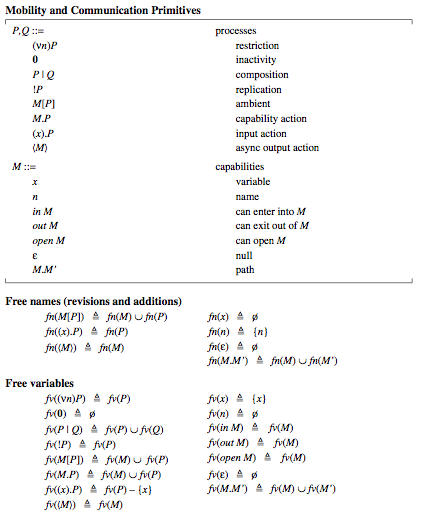
\includegraphics[scale=1]{ambient.png}
  \end{center}
  \captionsetup{justification=centering}  
  \caption{Syntax and scope in the ambient-calculus \\ -- \citep{Cardelli98mobileambients}}
  \label{ambient-syn}
\end{table}

\begin{table} [p]
  \begin{center}
  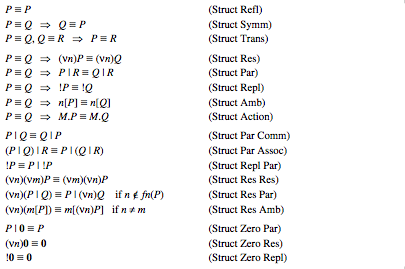
\includegraphics[scale=1]{ambient_str_1.png}
  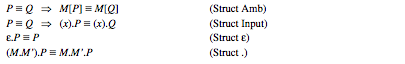
\includegraphics[scale=1]{ambient_str_2.png}
  \end{center}
  \captionsetup{justification=centering}    
  \caption{Structure congurence in the ambient-calculus \\ -- \citep{Cardelli98mobileambients}}
  \label{ambient-str}
\end{table}

\begin{table} [p]
  \begin{center}
  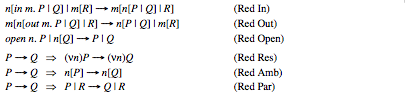
\includegraphics[scale=1]{ambient_red_1.png}
  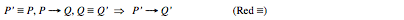
\includegraphics[scale=1]{ambient_red_2.png}
  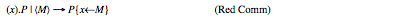
\includegraphics[scale=1]{ambient_red_3.png}
  \end{center}
  \captionsetup{justification=centering}    
  \caption{Reduction in the ambient-calculus \\ -- \citep{Cardelli98mobileambients}}
  \label{ambient-red}
\end{table}

\subsubsection{The Obliq Programming Language}
At the time of writing this report, there is no real language that implements the ambient-calculus\footnote{\citet{VMAmbient} proposed a virtual machine for the ambient calculus.}.  Instead,  this section will introduce the Obliq language, which has certain notions of ambient and influenced the design of the ambient calculus.

Obliq\citep{obliq} is one of the earliest programming languages which support distributed programming.  The language was designed before the pervasive of web applications.  It only supports simple object model which is a collection of fields.  Each field of an Obliq object could be a value (a constant or a procedure), a method, or an alias to an object.  An object could either be constructed directly by specifying its fields, or be cloned from other objects.  

The four operations which could be performed on objects are:
\begin{itemize}
  \item selection: a value field of a object could be selected and transmitted over the web.  If the selected value is a constant, the value will be transmitted.  By contrast, if the selected value is a method, values of its arguments will be transmitted to the remote site where the method is defined, the computation is performed remotely, and the result or an exception is returned to the site of the selection.
  \item updating: when an updating operation is performed on an remote object, the selected filed is updated to a value that might be sent across the web.  If the selected filed is a method, a transmission of method closure is required.
  \item cloning: cloning an object will yield a new object which contains all fields of argument objects or raise an error if field names of argument objects conflict.
  \item aliasing:  After executing an aliasing method, a.x := $\bf{alias}$ y $\bf{of}$ b $\bf{end}$, further operations on x of a will be redirected to y of b.
\end{itemize}

It is important to note that Obliq, as some other languages in the pre-web era, does not distinguish local values from distributed values.  By contrast, \citet{dis_note} pointed out that distinct views must be adopted for local and distributed objects, due to differences in latency, memory access, partial failure, and concurrency.
% \subsection{Type-parameterized Actor libraries}



% \subsection{Reliability Studies}

\section{Summing Up}

To review, the Actor Model \citep{Hewitt:1973} is proposed for designing 
concurrent systems. It is employed by Erlang  \citep{ArmstrongErlang} and other 
programming languages. Erlang developers designed the Supervision Principle in 
1998 when the Erlang/OTP library was released as an open-source project.  With 
the supervision principle, actors are supervised by their supervisors, who are 
responsible for initializing and monitoring their children.  Erlang developers 
claimed that applications using the supervision principle have achieved a 
high availability \citep{ArmstrongAXD}. Recently, the actor programming model 
and the supervision principle have been ported to Akka, an Actor library 
written in Scala.  Although Scala is a statically typed language and provides a 
sophisticated type system, the type of messages sent to Akka actors are 
dynamically checked when they are processed.  The next chapter presents the 
design and implementation of the TAkka library where type checks are involved
at the earliest opportunity to expose type errors.




